% Options for packages loaded elsewhere
\PassOptionsToPackage{unicode}{hyperref}
\PassOptionsToPackage{hyphens}{url}
%
\documentclass[
]{article}
\usepackage{amsmath,amssymb}
\usepackage{lmodern}
\usepackage{iftex}
\ifPDFTeX
  \usepackage[T1]{fontenc}
  \usepackage[utf8]{inputenc}
  \usepackage{textcomp} % provide euro and other symbols
\else % if luatex or xetex
  \usepackage{unicode-math}
  \defaultfontfeatures{Scale=MatchLowercase}
  \defaultfontfeatures[\rmfamily]{Ligatures=TeX,Scale=1}
\fi
% Use upquote if available, for straight quotes in verbatim environments
\IfFileExists{upquote.sty}{\usepackage{upquote}}{}
\IfFileExists{microtype.sty}{% use microtype if available
  \usepackage[]{microtype}
  \UseMicrotypeSet[protrusion]{basicmath} % disable protrusion for tt fonts
}{}
\makeatletter
\@ifundefined{KOMAClassName}{% if non-KOMA class
  \IfFileExists{parskip.sty}{%
    \usepackage{parskip}
  }{% else
    \setlength{\parindent}{0pt}
    \setlength{\parskip}{6pt plus 2pt minus 1pt}}
}{% if KOMA class
  \KOMAoptions{parskip=half}}
\makeatother
\usepackage{xcolor}
\IfFileExists{xurl.sty}{\usepackage{xurl}}{} % add URL line breaks if available
\IfFileExists{bookmark.sty}{\usepackage{bookmark}}{\usepackage{hyperref}}
\hypersetup{
  hidelinks,
  pdfcreator={LaTeX via pandoc}}
\urlstyle{same} % disable monospaced font for URLs
\usepackage[margin=1in]{geometry}
\usepackage{color}
\usepackage{fancyvrb}
\newcommand{\VerbBar}{|}
\newcommand{\VERB}{\Verb[commandchars=\\\{\}]}
\DefineVerbatimEnvironment{Highlighting}{Verbatim}{commandchars=\\\{\}}
% Add ',fontsize=\small' for more characters per line
\newenvironment{Shaded}{}{}
\newcommand{\AlertTok}[1]{\textcolor[rgb]{1.00,0.00,0.00}{#1}}
\newcommand{\AnnotationTok}[1]{\textcolor[rgb]{0.00,0.50,0.00}{#1}}
\newcommand{\AttributeTok}[1]{#1}
\newcommand{\BaseNTok}[1]{#1}
\newcommand{\BuiltInTok}[1]{#1}
\newcommand{\CharTok}[1]{\textcolor[rgb]{0.00,0.50,0.50}{#1}}
\newcommand{\CommentTok}[1]{\textcolor[rgb]{0.00,0.50,0.00}{#1}}
\newcommand{\CommentVarTok}[1]{\textcolor[rgb]{0.00,0.50,0.00}{#1}}
\newcommand{\ConstantTok}[1]{#1}
\newcommand{\ControlFlowTok}[1]{\textcolor[rgb]{0.00,0.00,1.00}{#1}}
\newcommand{\DataTypeTok}[1]{#1}
\newcommand{\DecValTok}[1]{#1}
\newcommand{\DocumentationTok}[1]{\textcolor[rgb]{0.00,0.50,0.00}{#1}}
\newcommand{\ErrorTok}[1]{\textcolor[rgb]{1.00,0.00,0.00}{\textbf{#1}}}
\newcommand{\ExtensionTok}[1]{#1}
\newcommand{\FloatTok}[1]{#1}
\newcommand{\FunctionTok}[1]{#1}
\newcommand{\ImportTok}[1]{#1}
\newcommand{\InformationTok}[1]{\textcolor[rgb]{0.00,0.50,0.00}{#1}}
\newcommand{\KeywordTok}[1]{\textcolor[rgb]{0.00,0.00,1.00}{#1}}
\newcommand{\NormalTok}[1]{#1}
\newcommand{\OperatorTok}[1]{#1}
\newcommand{\OtherTok}[1]{\textcolor[rgb]{1.00,0.25,0.00}{#1}}
\newcommand{\PreprocessorTok}[1]{\textcolor[rgb]{1.00,0.25,0.00}{#1}}
\newcommand{\RegionMarkerTok}[1]{#1}
\newcommand{\SpecialCharTok}[1]{\textcolor[rgb]{0.00,0.50,0.50}{#1}}
\newcommand{\SpecialStringTok}[1]{\textcolor[rgb]{0.00,0.50,0.50}{#1}}
\newcommand{\StringTok}[1]{\textcolor[rgb]{0.00,0.50,0.50}{#1}}
\newcommand{\VariableTok}[1]{#1}
\newcommand{\VerbatimStringTok}[1]{\textcolor[rgb]{0.00,0.50,0.50}{#1}}
\newcommand{\WarningTok}[1]{\textcolor[rgb]{0.00,0.50,0.00}{\textbf{#1}}}
\usepackage{longtable,booktabs,array}
\usepackage{calc} % for calculating minipage widths
% Correct order of tables after \paragraph or \subparagraph
\usepackage{etoolbox}
\makeatletter
\patchcmd\longtable{\par}{\if@noskipsec\mbox{}\fi\par}{}{}
\makeatother
% Allow footnotes in longtable head/foot
\IfFileExists{footnotehyper.sty}{\usepackage{footnotehyper}}{\usepackage{footnote}}
\makesavenoteenv{longtable}
\usepackage{graphicx}
\makeatletter
\def\maxwidth{\ifdim\Gin@nat@width>\linewidth\linewidth\else\Gin@nat@width\fi}
\def\maxheight{\ifdim\Gin@nat@height>\textheight\textheight\else\Gin@nat@height\fi}
\makeatother
% Scale images if necessary, so that they will not overflow the page
% margins by default, and it is still possible to overwrite the defaults
% using explicit options in \includegraphics[width, height, ...]{}
\setkeys{Gin}{width=\maxwidth,height=\maxheight,keepaspectratio}
% Set default figure placement to htbp
\makeatletter
\def\fps@figure{htbp}
\makeatother
\setlength{\emergencystretch}{3em} % prevent overfull lines
\providecommand{\tightlist}{%
  \setlength{\itemsep}{0pt}\setlength{\parskip}{0pt}}
\setcounter{secnumdepth}{-\maxdimen} % remove section numbering
\usepackage{sectsty}
\subsectionfont{\color{cyan}}
\usepackage{titling}
\pretitle{\begin{center} \includegraphics[width=2in,height=2in]{mccombs.png}\LARGE\\}
\posttitle{\end{center}}
\ifLuaTeX
  \usepackage{selnolig}  % disable illegal ligatures
\fi

\author{}
\date{\vspace{-2.5em}}

\begin{document}

\begin{longtable}[]{@{}l@{}}
\toprule
\endhead
\textbf{Introduction to Machine Learning Take Home Exam} \\
\textbf{Author: Disha Gandhi} \\
\textbf{Date: 07/21/2021} \\
\bottomrule
\end{longtable}

\hypertarget{chapter-2-question-10}{%
\subsection{CHAPTER 2 \textasciitilde{} QUESTION
10}\label{chapter-2-question-10}}

\hypertarget{part-a}{%
\paragraph{PART A}\label{part-a}}

The Boston dataset is as follows

\begin{verbatim}
##      crim zn indus chas   nox    rm  age    dis rad tax ptratio  black lstat
## 1 0.00632 18  2.31    0 0.538 6.575 65.2 4.0900   1 296    15.3 396.90  4.98
## 2 0.02731  0  7.07    0 0.469 6.421 78.9 4.9671   2 242    17.8 396.90  9.14
## 3 0.02729  0  7.07    0 0.469 7.185 61.1 4.9671   2 242    17.8 392.83  4.03
## 4 0.03237  0  2.18    0 0.458 6.998 45.8 6.0622   3 222    18.7 394.63  2.94
## 5 0.06905  0  2.18    0 0.458 7.147 54.2 6.0622   3 222    18.7 396.90  5.33
## 6 0.02985  0  2.18    0 0.458 6.430 58.7 6.0622   3 222    18.7 394.12  5.21
##   medv
## 1 24.0
## 2 21.6
## 3 34.7
## 4 33.4
## 5 36.2
## 6 28.7
\end{verbatim}

\begin{verbatim}
## [1] "The number of columns in this dataset are 14"
\end{verbatim}

\begin{verbatim}
## [1] "The number of rows in this dataset are 506"
\end{verbatim}

The rows represent neighbourhoods in Boston for housing and the columns
represent further details about each of those neighbourhoods which will
act as predictors/features too when we want to predict one of those
features.

\pagebreak

\hypertarget{part-b}{%
\paragraph{PART B}\label{part-b}}

\begin{center}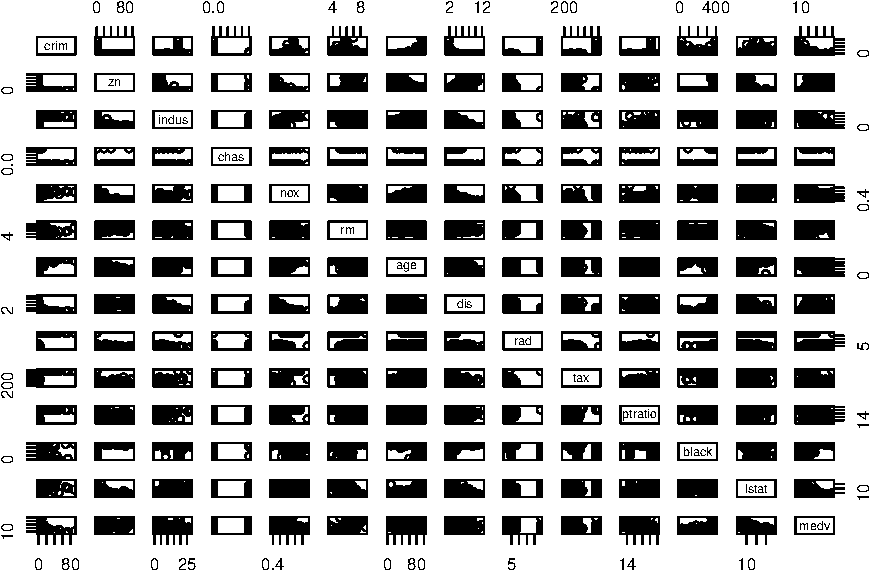
\includegraphics{Disha_Gandhi_Take_Home_Exam_PDF_files/figure-latex/unnamed-chunk-2-1} \end{center}

\begin{verbatim}
##          crim    zn indus  chas   nox    rm   age   dis   rad   tax ptratio
## crim     1.00 -0.20  0.41 -0.06  0.42 -0.22  0.35 -0.38  0.63  0.58    0.29
## zn      -0.20  1.00 -0.53 -0.04 -0.52  0.31 -0.57  0.66 -0.31 -0.31   -0.39
## indus    0.41 -0.53  1.00  0.06  0.76 -0.39  0.64 -0.71  0.60  0.72    0.38
## chas    -0.06 -0.04  0.06  1.00  0.09  0.09  0.09 -0.10 -0.01 -0.04   -0.12
## nox      0.42 -0.52  0.76  0.09  1.00 -0.30  0.73 -0.77  0.61  0.67    0.19
## rm      -0.22  0.31 -0.39  0.09 -0.30  1.00 -0.24  0.21 -0.21 -0.29   -0.36
## age      0.35 -0.57  0.64  0.09  0.73 -0.24  1.00 -0.75  0.46  0.51    0.26
## dis     -0.38  0.66 -0.71 -0.10 -0.77  0.21 -0.75  1.00 -0.49 -0.53   -0.23
## rad      0.63 -0.31  0.60 -0.01  0.61 -0.21  0.46 -0.49  1.00  0.91    0.46
## tax      0.58 -0.31  0.72 -0.04  0.67 -0.29  0.51 -0.53  0.91  1.00    0.46
## ptratio  0.29 -0.39  0.38 -0.12  0.19 -0.36  0.26 -0.23  0.46  0.46    1.00
## black   -0.39  0.18 -0.36  0.05 -0.38  0.13 -0.27  0.29 -0.44 -0.44   -0.18
## lstat    0.46 -0.41  0.60 -0.05  0.59 -0.61  0.60 -0.50  0.49  0.54    0.37
## medv    -0.39  0.36 -0.48  0.18 -0.43  0.70 -0.38  0.25 -0.38 -0.47   -0.51
##         black lstat  medv
## crim    -0.39  0.46 -0.39
## zn       0.18 -0.41  0.36
## indus   -0.36  0.60 -0.48
## chas     0.05 -0.05  0.18
## nox     -0.38  0.59 -0.43
## rm       0.13 -0.61  0.70
## age     -0.27  0.60 -0.38
## dis      0.29 -0.50  0.25
## rad     -0.44  0.49 -0.38
## tax     -0.44  0.54 -0.47
## ptratio -0.18  0.37 -0.51
## black    1.00 -0.37  0.33
## lstat   -0.37  1.00 -0.74
## medv     0.33 -0.74  1.00
\end{verbatim}

Along with pairwise scatterplot I have also drawn the correlation matrix
to get a better clarity of the features. We can observe over here that

-- There is a \textbf{strong positive correlation} between \textbf{tax
and indus, tax and nox, tax and rad, crim and rad, nox and rad, zn and
dis, indus and age, nox and age, medv and rm, nox and indus.}

-- There is a \textbf{strong negative correlation} between \textbf{dis
and indus, nox and dis, rm and lstat, dis and age, dis and nox, lstat
and medv.}

-- There is a \textbf{very small positive correlation} between
\textbf{crim and indus, crim and nox, crim and tax, crim and lstat, zn
and rm, zn and medv, indus and ptratio, nox and crim, nox and lstat, age
and crim, age and rad, age and tax, rad and ptratio, rad and lstat, tax
and ptratio, tax and lstat, ptratio and lstat, black and medv, medv and
zn.}

-- There is a \textbf{very small negative correlation} between
\textbf{crim and dis, crim and black, crim and medv, zn and indus, zn
and nox, zn and age, zn and rad, zn and tax, zn and ptratio, zn and
lstat, indus and rm, indus and black, indus and medv, nox and zn, nox
and rm, nox and black, nox and medv, rm and ptratio, age and medv, dis
and crim, dis and rad, dis and tax, dis and lstat, rad and black, rad
and medv, tax and black, tax and medv, ptratio and medv, black and
lstat, black and lstat.}

\begin{itemize}
\tightlist
\item
  A negative correlation implies inverse proportionality and a positive
  correlation implies direct proportionality.
\item
  I made all the above assessments using graphs and correlation matrix.
\end{itemize}

\pagebreak

\hypertarget{part-c}{%
\paragraph{PART C}\label{part-c}}

\begin{center}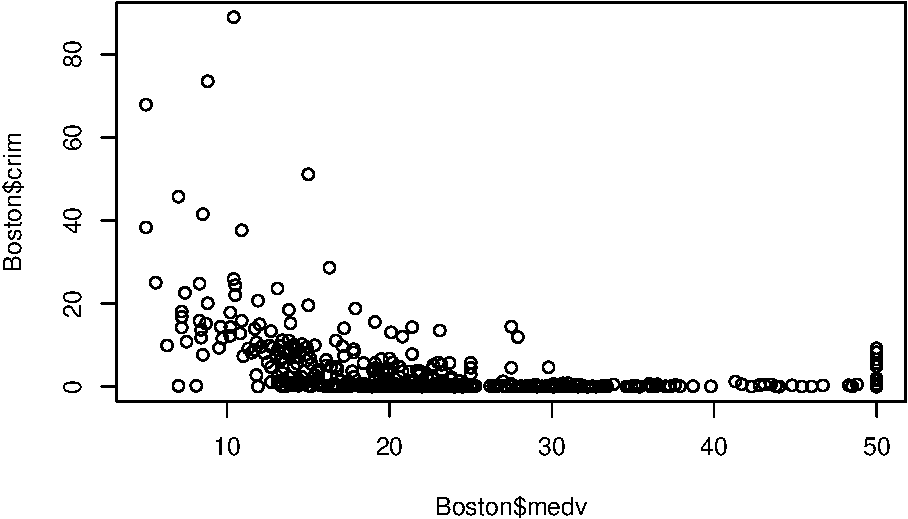
\includegraphics{Disha_Gandhi_Take_Home_Exam_PDF_files/figure-latex/unnamed-chunk-3-1} \end{center}

The more expensive the homes, less crime because enhanced security

\begin{center}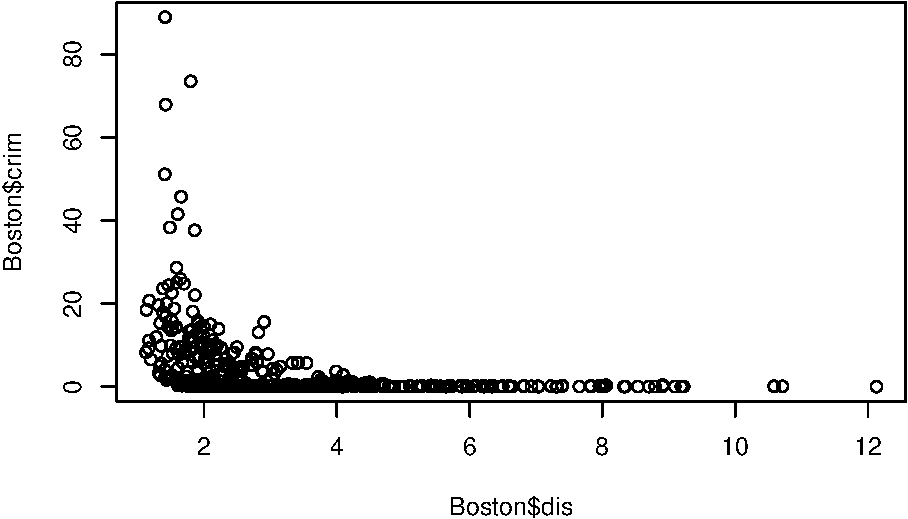
\includegraphics{Disha_Gandhi_Take_Home_Exam_PDF_files/figure-latex/unnamed-chunk-4-1} \end{center}

The Closer to work-area, it will be less crime because it will be a
densely populated area

\begin{center}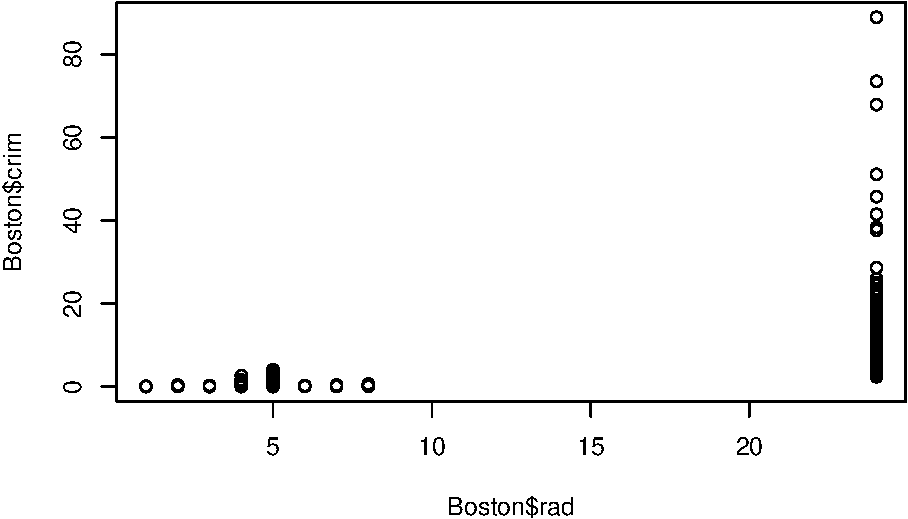
\includegraphics{Disha_Gandhi_Take_Home_Exam_PDF_files/figure-latex/unnamed-chunk-5-1} \end{center}

Higher index of accessibility to radial highways implies more crime
because home are now farther from accessible areas.

\begin{center}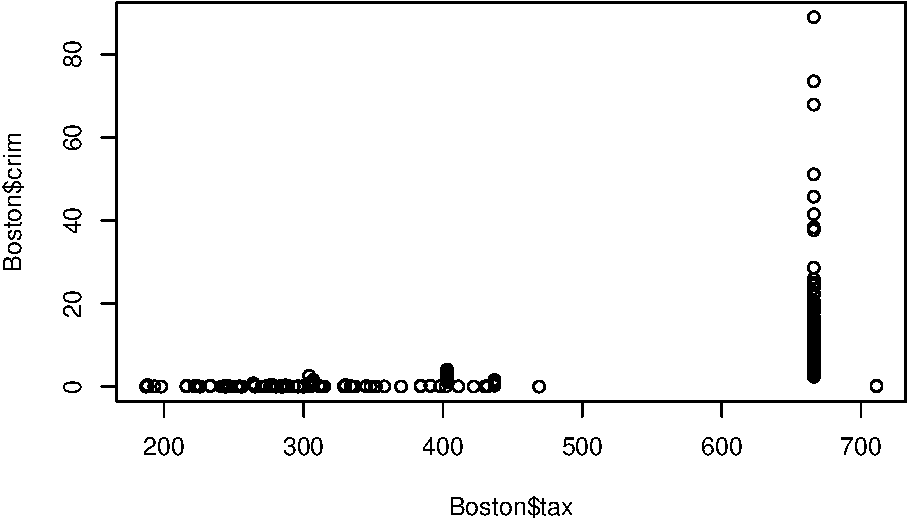
\includegraphics{Disha_Gandhi_Take_Home_Exam_PDF_files/figure-latex/unnamed-chunk-6-1} \end{center}

Higher tax rate, more crime

\begin{center}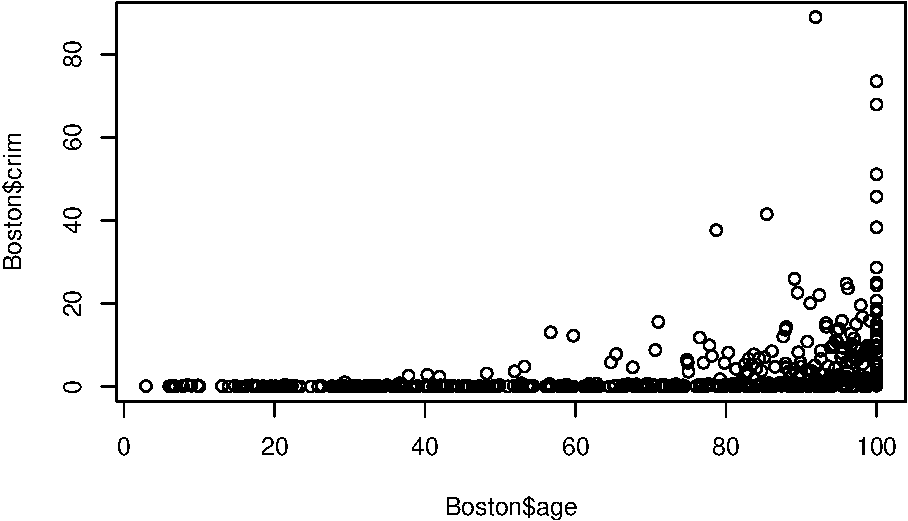
\includegraphics{Disha_Gandhi_Take_Home_Exam_PDF_files/figure-latex/unnamed-chunk-7-1} \end{center}

Older homes mean more crime

\begin{itemize}
\tightlist
\item
  I took only some features here based on the correlation score I
  received for them from above part. Selecting the ones with little or
  significant correlation.
\end{itemize}

\pagebreak

\hypertarget{part-d}{%
\paragraph{PART D}\label{part-d}}

\begin{center}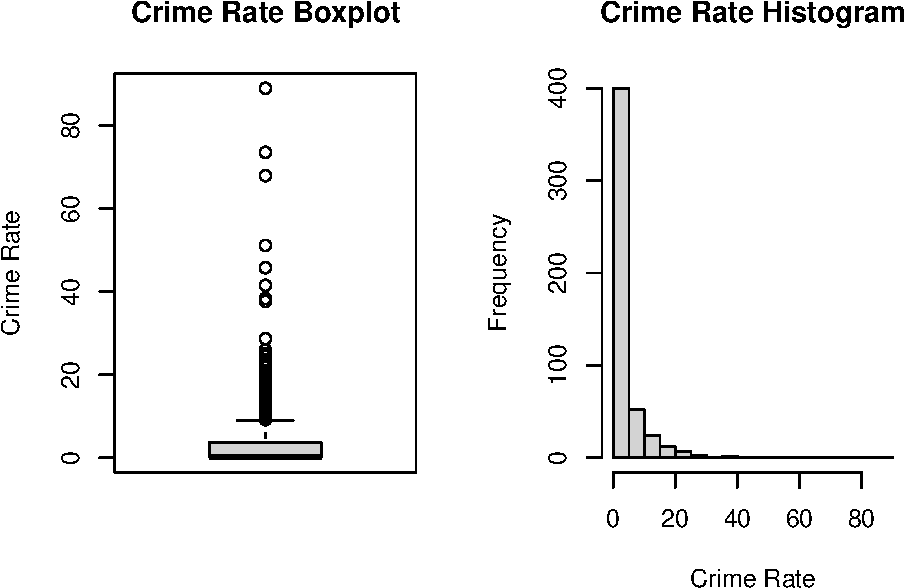
\includegraphics{Disha_Gandhi_Take_Home_Exam_PDF_files/figure-latex/unnamed-chunk-8-1} \end{center}

\begin{verbatim}
##     Min.  1st Qu.   Median     Mean  3rd Qu.     Max. 
##  0.00632  0.08204  0.25651  3.61352  3.67708 88.97620
\end{verbatim}

\begin{itemize}
\tightlist
\item
  We can clearly see from above insights on Crime Rate that maximum or a
  large portion of Suburbs have their crime concentrated in between 0
  and 1 and so there are very less suburbs going near the max value of
  88.97. But they are a good significant ones. In the box plot we can
  clearly see that there are so many outliers which are present above
  the IQR which gives us a hint already that this feature does not
  follow normal distribution.
\end{itemize}

\begin{verbatim}
## [1] "The number of suburbs in this dataset that have a crime rate of greater than 30 are 8"
\end{verbatim}

\begin{itemize}
\tightlist
\item
  There are 8 suburbs that have crime rate stretching in the range
  30-90. So these few suburbs should be taken into consideration to make
  them more hospitable and safe. These suburbs are causing the mean to
  increase to 3.6 because we can see that the median is still at 0.25,
  implying the majority concentration is less than 1.
\end{itemize}

\begin{center}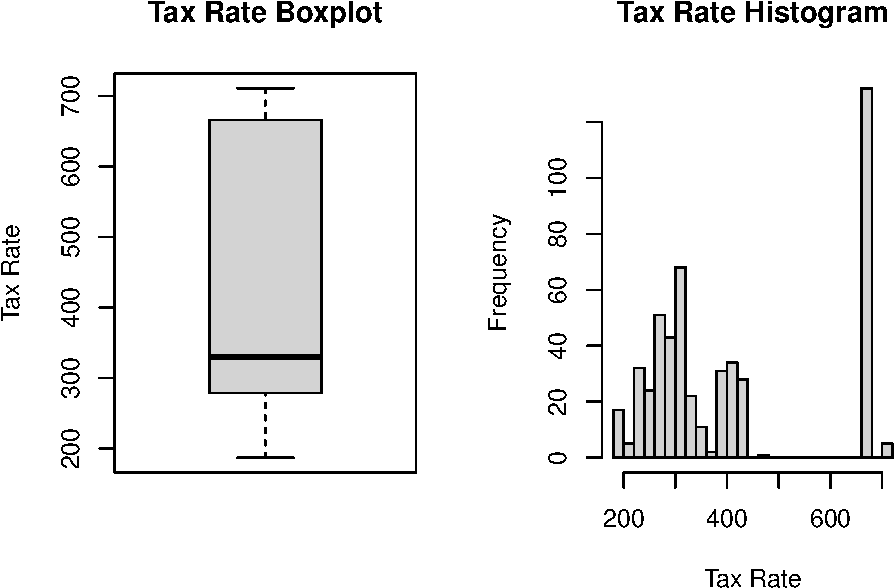
\includegraphics{Disha_Gandhi_Take_Home_Exam_PDF_files/figure-latex/unnamed-chunk-10-1} \end{center}

\begin{verbatim}
##    Min. 1st Qu.  Median    Mean 3rd Qu.    Max. 
##   187.0   279.0   330.0   408.2   666.0   711.0
\end{verbatim}

\begin{itemize}
\tightlist
\item
  The insights above on tax rate show that we can clearly seperate
  suburbs with low tax rates and high tax rates. Since the mean and
  median are not so far and there are no outliers we can assess that
  there are no extreme values. We can also see from the histogram that
  there are a lot of suburbs in the range of 650-800 and so we can state
  that some suburbs have a particularly high tax rate though not beyond
  the IQR and hence in the satifactory range. But yes there is a clear
  cut division between low taxed suburbs and high ones.
\end{itemize}

\begin{center}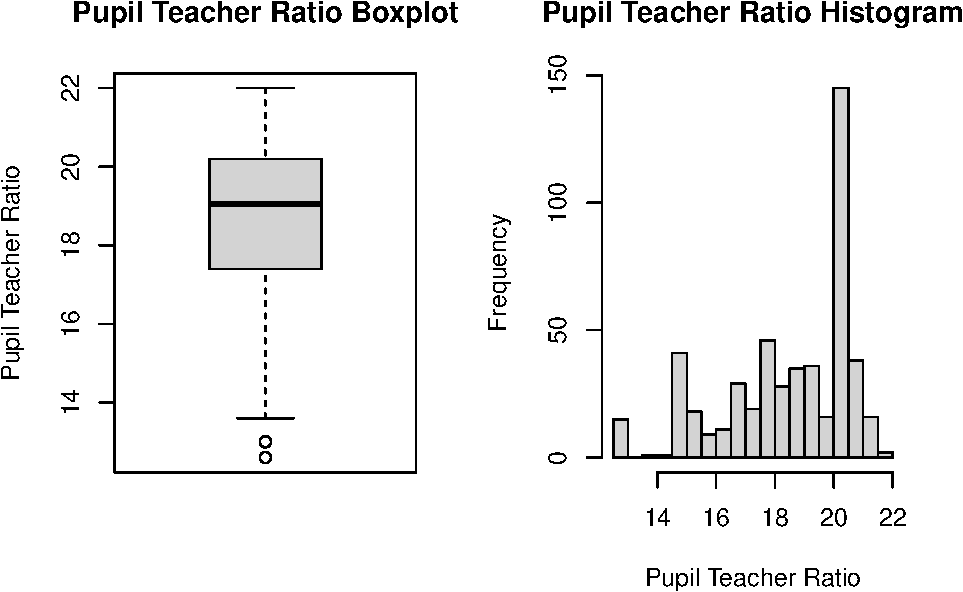
\includegraphics{Disha_Gandhi_Take_Home_Exam_PDF_files/figure-latex/unnamed-chunk-11-1} \end{center}

\begin{verbatim}
##    Min. 1st Qu.  Median    Mean 3rd Qu.    Max. 
##   12.60   17.40   19.05   18.46   20.20   22.00
\end{verbatim}

\begin{itemize}
\tightlist
\item
  The insights above on pupil teacher ratio show that there is clearly
  no suburb having particularly high pupil teacher ratio, though are two
  having particularly low pupil teacher ratio. There are also some good
  number of them in the third quartile but since they are not causing a
  huge variation in the distribution we can not declare them as
  particularly high. The histogram says that the maximum suburbs are in
  the bucket of 20 but that is still not the maximum. The maximum is at
  22. Hence no major extreme can be seen for this feature.
\end{itemize}

\pagebreak

\hypertarget{part-e}{%
\paragraph{PART E}\label{part-e}}

\begin{verbatim}
## [1] "The number of suburbs in this dataset bounding the charles river are 35"
\end{verbatim}

\hypertarget{part-f}{%
\paragraph{PART F}\label{part-f}}

\begin{verbatim}
## [1] "The median pupil-teacher ratio of the suburbs in this town is 19.05"
\end{verbatim}

\hypertarget{part-g}{%
\paragraph{PART G}\label{part-g}}

There are two suburbs which have the lowest median value of owner
occupied homes which is 5. Below are the values of other predictors for
it.

\begin{verbatim}
##        crim zn indus chas   nox    rm age    dis rad tax ptratio  black lstat
## 399 38.3518  0  18.1    0 0.693 5.453 100 1.4896  24 666    20.2 396.90 30.59
## 406 67.9208  0  18.1    0 0.693 5.683 100 1.4254  24 666    20.2 384.97 22.98
##     medv
## 399    5
## 406    5
\end{verbatim}

Let us look at the summary of the dataset to compare the above two
suburbs.

\begin{verbatim}
##       crim                zn             indus            chas        
##  Min.   : 0.00632   Min.   :  0.00   Min.   : 0.46   Min.   :0.00000  
##  1st Qu.: 0.08205   1st Qu.:  0.00   1st Qu.: 5.19   1st Qu.:0.00000  
##  Median : 0.25651   Median :  0.00   Median : 9.69   Median :0.00000  
##  Mean   : 3.61352   Mean   : 11.36   Mean   :11.14   Mean   :0.06917  
##  3rd Qu.: 3.67708   3rd Qu.: 12.50   3rd Qu.:18.10   3rd Qu.:0.00000  
##  Max.   :88.97620   Max.   :100.00   Max.   :27.74   Max.   :1.00000  
##       nox               rm             age              dis        
##  Min.   :0.3850   Min.   :3.561   Min.   :  2.90   Min.   : 1.130  
##  1st Qu.:0.4490   1st Qu.:5.886   1st Qu.: 45.02   1st Qu.: 2.100  
##  Median :0.5380   Median :6.208   Median : 77.50   Median : 3.207  
##  Mean   :0.5547   Mean   :6.285   Mean   : 68.57   Mean   : 3.795  
##  3rd Qu.:0.6240   3rd Qu.:6.623   3rd Qu.: 94.08   3rd Qu.: 5.188  
##  Max.   :0.8710   Max.   :8.780   Max.   :100.00   Max.   :12.127  
##       rad              tax           ptratio          black       
##  Min.   : 1.000   Min.   :187.0   Min.   :12.60   Min.   :  0.32  
##  1st Qu.: 4.000   1st Qu.:279.0   1st Qu.:17.40   1st Qu.:375.38  
##  Median : 5.000   Median :330.0   Median :19.05   Median :391.44  
##  Mean   : 9.549   Mean   :408.2   Mean   :18.46   Mean   :356.67  
##  3rd Qu.:24.000   3rd Qu.:666.0   3rd Qu.:20.20   3rd Qu.:396.23  
##  Max.   :24.000   Max.   :711.0   Max.   :22.00   Max.   :396.90  
##      lstat            medv      
##  Min.   : 1.73   Min.   : 5.00  
##  1st Qu.: 6.95   1st Qu.:17.02  
##  Median :11.36   Median :21.20  
##  Mean   :12.65   Mean   :22.53  
##  3rd Qu.:16.95   3rd Qu.:25.00  
##  Max.   :37.97   Max.   :50.00
\end{verbatim}

We can see that

-- The crime rate(crim) for both of these suburbs is \textbf{above 3rd
quartile.}

-- The proportion of residential land zone(zn) is \textbf{minimum value}
for both of them.

-- The proportion of non retail business acres per town(indus) is
\textbf{at the 3rd quartile.}

-- The charles river bounding(chas) is \textbf{not present} for both.

-- The nitrogen oxide concentration(nox) is \textbf{above 3rd quartile}
for both.

-- The average number of rooms per dwelling(rm) for both is \textbf{less
than 1st quartile.}

-- The age of the house(age) is \textbf{maximum} for them i.e both are
very old suburbs.

-- The distance from employment centres(dis) for both the suburbs is
\textbf{less than 1st quartile.}

-- The accessibility to radial highways(rad) is \textbf{maximum} for
both.

-- The property tax(tax) in these suburbs is \textbf{at 3rd quartile.}

-- The pupil teacher ratio(pt ratio) in these suburbs is \textbf{at 3rd
quartile} for both of them.

-- The black population(black) is at \textbf{maximum} for 1st suburb and
\textbf{above 1st quartile} for 2nd suburb.

-- The population of lower status people(lstat) is \textbf{above 3rd
quartile} for both of the suburbs.

-- The median value of owner occupied homes(medv) is for obvious reasons
at \textbf{minimum} for both.

\pagebreak

\hypertarget{part-h}{%
\paragraph{PART H}\label{part-h}}

\begin{verbatim}
## [1] "The number of suburbs in this dataset having more than 7 rooms per dwelling in average is 64"
\end{verbatim}

\begin{verbatim}
## [1] "The number of suburbs in this dataset having more than 8 rooms per dwelling in average is 13"
\end{verbatim}

Let us look at those 13 suburbs having more than 8 rooms per dwelling in
average

\begin{verbatim}
##       crim               zn            indus             chas       
##  Min.   :0.02009   Min.   : 0.00   Min.   : 2.680   Min.   :0.0000  
##  1st Qu.:0.33147   1st Qu.: 0.00   1st Qu.: 3.970   1st Qu.:0.0000  
##  Median :0.52014   Median : 0.00   Median : 6.200   Median :0.0000  
##  Mean   :0.71879   Mean   :13.62   Mean   : 7.078   Mean   :0.1538  
##  3rd Qu.:0.57834   3rd Qu.:20.00   3rd Qu.: 6.200   3rd Qu.:0.0000  
##  Max.   :3.47428   Max.   :95.00   Max.   :19.580   Max.   :1.0000  
##       nox               rm             age             dis       
##  Min.   :0.4161   Min.   :8.034   Min.   : 8.40   Min.   :1.801  
##  1st Qu.:0.5040   1st Qu.:8.247   1st Qu.:70.40   1st Qu.:2.288  
##  Median :0.5070   Median :8.297   Median :78.30   Median :2.894  
##  Mean   :0.5392   Mean   :8.349   Mean   :71.54   Mean   :3.430  
##  3rd Qu.:0.6050   3rd Qu.:8.398   3rd Qu.:86.50   3rd Qu.:3.652  
##  Max.   :0.7180   Max.   :8.780   Max.   :93.90   Max.   :8.907  
##       rad              tax           ptratio          black      
##  Min.   : 2.000   Min.   :224.0   Min.   :13.00   Min.   :354.6  
##  1st Qu.: 5.000   1st Qu.:264.0   1st Qu.:14.70   1st Qu.:384.5  
##  Median : 7.000   Median :307.0   Median :17.40   Median :386.9  
##  Mean   : 7.462   Mean   :325.1   Mean   :16.36   Mean   :385.2  
##  3rd Qu.: 8.000   3rd Qu.:307.0   3rd Qu.:17.40   3rd Qu.:389.7  
##  Max.   :24.000   Max.   :666.0   Max.   :20.20   Max.   :396.9  
##      lstat           medv     
##  Min.   :2.47   Min.   :21.9  
##  1st Qu.:3.32   1st Qu.:41.7  
##  Median :4.14   Median :48.3  
##  Mean   :4.31   Mean   :44.2  
##  3rd Qu.:5.12   3rd Qu.:50.0  
##  Max.   :7.44   Max.   :50.0
\end{verbatim}

We can see here that

\begin{itemize}
\item
  Crime rate is lower for these suburbs.
\item
  The population of blacks and lower status people is also comparatively
  high in these suburbs.
\item
  Rest all the features are almost of the same range
\end{itemize}

\pagebreak

\hypertarget{chapter-3-question-15}{%
\subsection{CHAPTER 3 \textasciitilde{} QUESTION
15}\label{chapter-3-question-15}}

\hypertarget{part-a-1}{%
\paragraph{PART A}\label{part-a-1}}

\hypertarget{single-predictor---zn}{%
\subparagraph{\texorpdfstring{\textbf{Single Predictor -
ZN}}{Single Predictor - ZN}}\label{single-predictor---zn}}

\begin{verbatim}
## 
## Call:
## lm(formula = crim ~ zn)
## 
## Residuals:
##    Min     1Q Median     3Q    Max 
## -4.429 -4.222 -2.620  1.250 84.523 
## 
## Coefficients:
##             Estimate Std. Error t value Pr(>|t|)    
## (Intercept)  4.45369    0.41722  10.675  < 2e-16 ***
## zn          -0.07393    0.01609  -4.594 5.51e-06 ***
## ---
## Signif. codes:  0 '***' 0.001 '**' 0.01 '*' 0.05 '.' 0.1 ' ' 1
## 
## Residual standard error: 8.435 on 504 degrees of freedom
## Multiple R-squared:  0.04019,    Adjusted R-squared:  0.03828 
## F-statistic:  21.1 on 1 and 504 DF,  p-value: 5.506e-06
\end{verbatim}

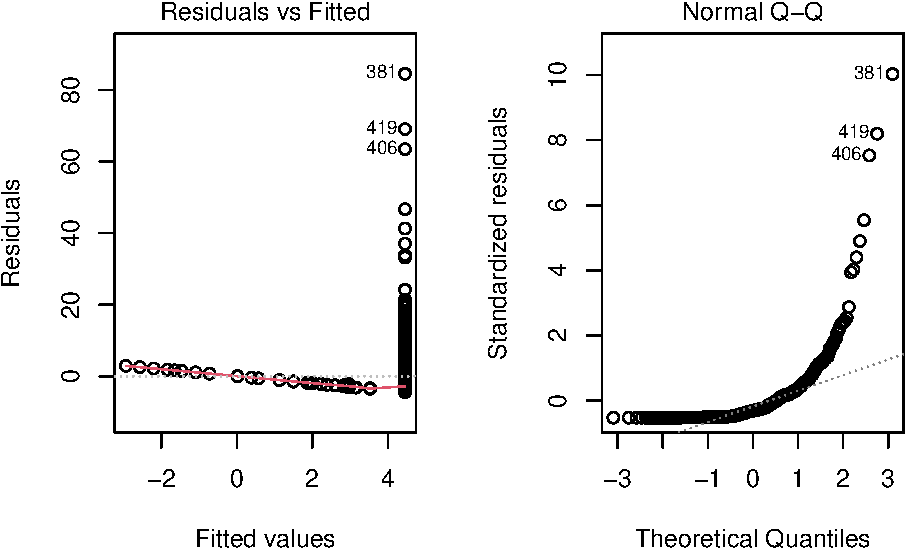
\includegraphics{Disha_Gandhi_Take_Home_Exam_PDF_files/figure-latex/unnamed-chunk-18-1.pdf}
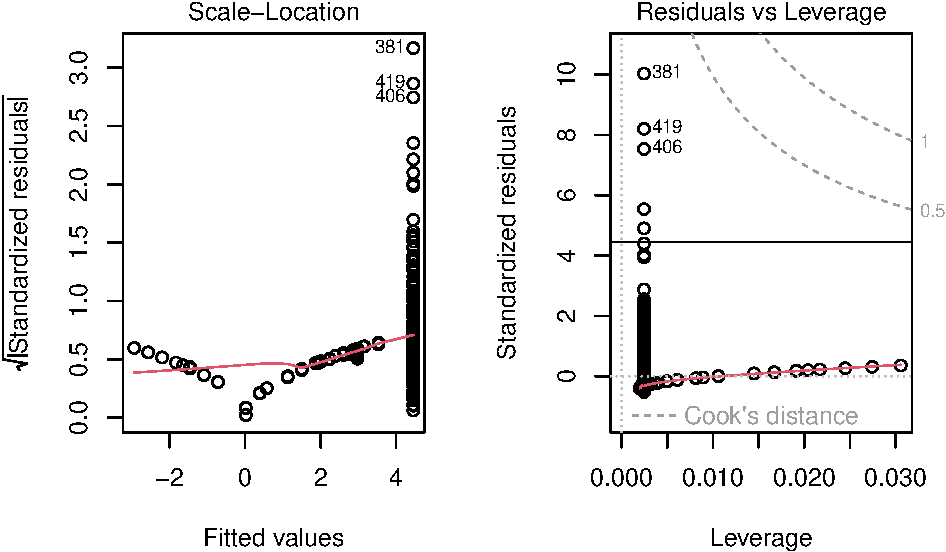
\includegraphics{Disha_Gandhi_Take_Home_Exam_PDF_files/figure-latex/unnamed-chunk-18-2.pdf}

\hypertarget{single-predictor---indus}{%
\subparagraph{\texorpdfstring{\textbf{Single Predictor -
INDUS}}{Single Predictor - INDUS}}\label{single-predictor---indus}}

\begin{verbatim}
## 
## Call:
## lm(formula = crim ~ indus)
## 
## Residuals:
##     Min      1Q  Median      3Q     Max 
## -11.972  -2.698  -0.736   0.712  81.813 
## 
## Coefficients:
##             Estimate Std. Error t value Pr(>|t|)    
## (Intercept) -2.06374    0.66723  -3.093  0.00209 ** 
## indus        0.50978    0.05102   9.991  < 2e-16 ***
## ---
## Signif. codes:  0 '***' 0.001 '**' 0.01 '*' 0.05 '.' 0.1 ' ' 1
## 
## Residual standard error: 7.866 on 504 degrees of freedom
## Multiple R-squared:  0.1653, Adjusted R-squared:  0.1637 
## F-statistic: 99.82 on 1 and 504 DF,  p-value: < 2.2e-16
\end{verbatim}

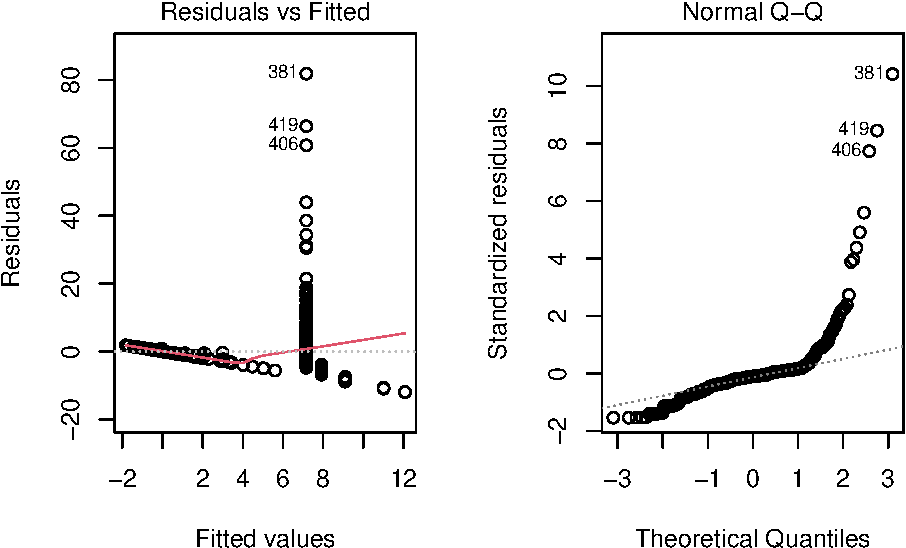
\includegraphics{Disha_Gandhi_Take_Home_Exam_PDF_files/figure-latex/unnamed-chunk-19-1.pdf}
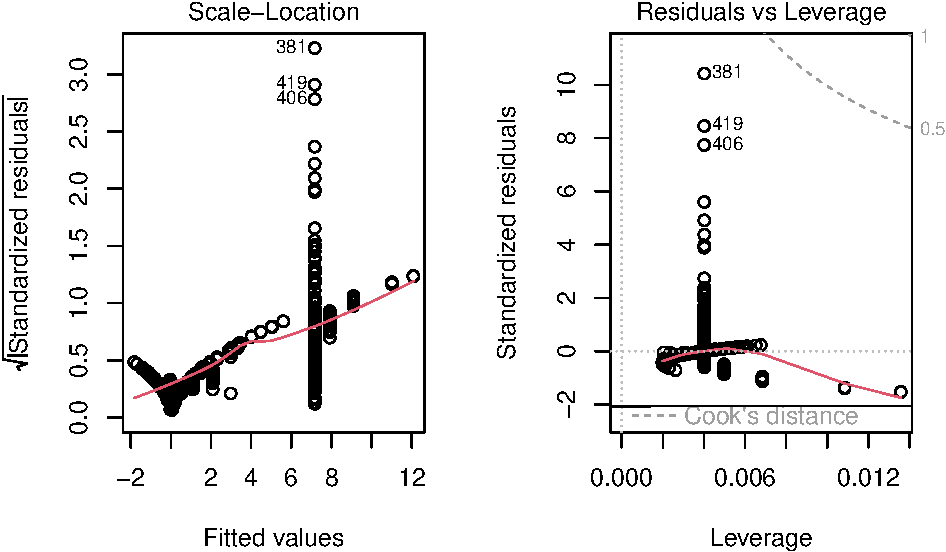
\includegraphics{Disha_Gandhi_Take_Home_Exam_PDF_files/figure-latex/unnamed-chunk-19-2.pdf}

\hypertarget{single-predictor---chas}{%
\subparagraph{\texorpdfstring{\textbf{Single Predictor -
CHAS}}{Single Predictor - CHAS}}\label{single-predictor---chas}}

\begin{verbatim}
## 
## Call:
## lm(formula = crim ~ chas)
## 
## Residuals:
##    Min     1Q Median     3Q    Max 
## -3.738 -3.661 -3.435  0.018 85.232 
## 
## Coefficients:
##             Estimate Std. Error t value Pr(>|t|)    
## (Intercept)   3.7444     0.3961   9.453   <2e-16 ***
## chas         -1.8928     1.5061  -1.257    0.209    
## ---
## Signif. codes:  0 '***' 0.001 '**' 0.01 '*' 0.05 '.' 0.1 ' ' 1
## 
## Residual standard error: 8.597 on 504 degrees of freedom
## Multiple R-squared:  0.003124,   Adjusted R-squared:  0.001146 
## F-statistic: 1.579 on 1 and 504 DF,  p-value: 0.2094
\end{verbatim}

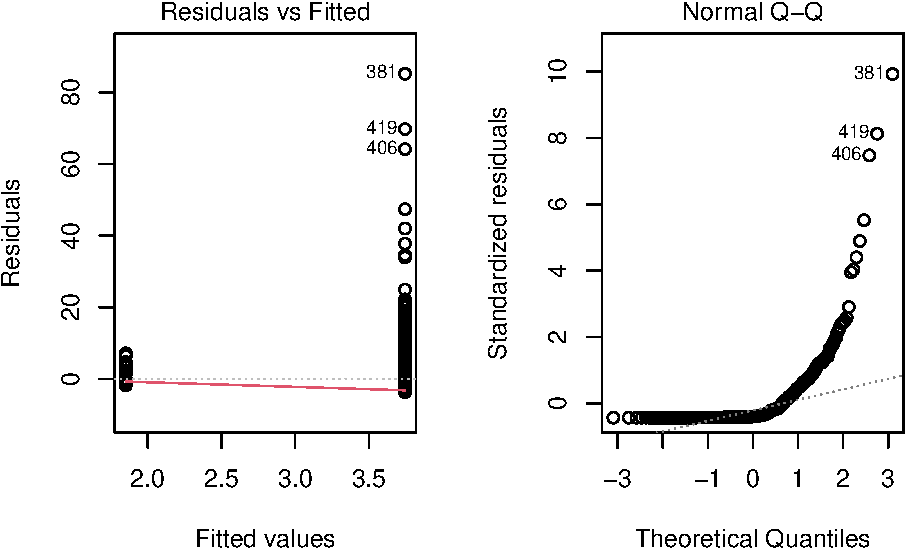
\includegraphics{Disha_Gandhi_Take_Home_Exam_PDF_files/figure-latex/unnamed-chunk-20-1.pdf}
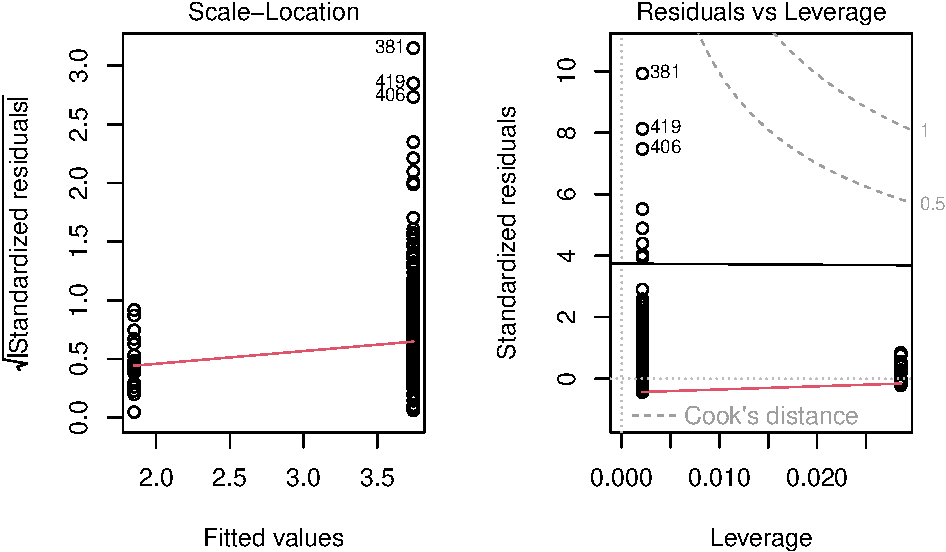
\includegraphics{Disha_Gandhi_Take_Home_Exam_PDF_files/figure-latex/unnamed-chunk-20-2.pdf}

\hypertarget{single-predictor---nox}{%
\subparagraph{\texorpdfstring{\textbf{Single Predictor -
NOX}}{Single Predictor - NOX}}\label{single-predictor---nox}}

\begin{verbatim}
## 
## Call:
## lm(formula = crim ~ nox)
## 
## Residuals:
##     Min      1Q  Median      3Q     Max 
## -12.371  -2.738  -0.974   0.559  81.728 
## 
## Coefficients:
##             Estimate Std. Error t value Pr(>|t|)    
## (Intercept)  -13.720      1.699  -8.073 5.08e-15 ***
## nox           31.249      2.999  10.419  < 2e-16 ***
## ---
## Signif. codes:  0 '***' 0.001 '**' 0.01 '*' 0.05 '.' 0.1 ' ' 1
## 
## Residual standard error: 7.81 on 504 degrees of freedom
## Multiple R-squared:  0.1772, Adjusted R-squared:  0.1756 
## F-statistic: 108.6 on 1 and 504 DF,  p-value: < 2.2e-16
\end{verbatim}

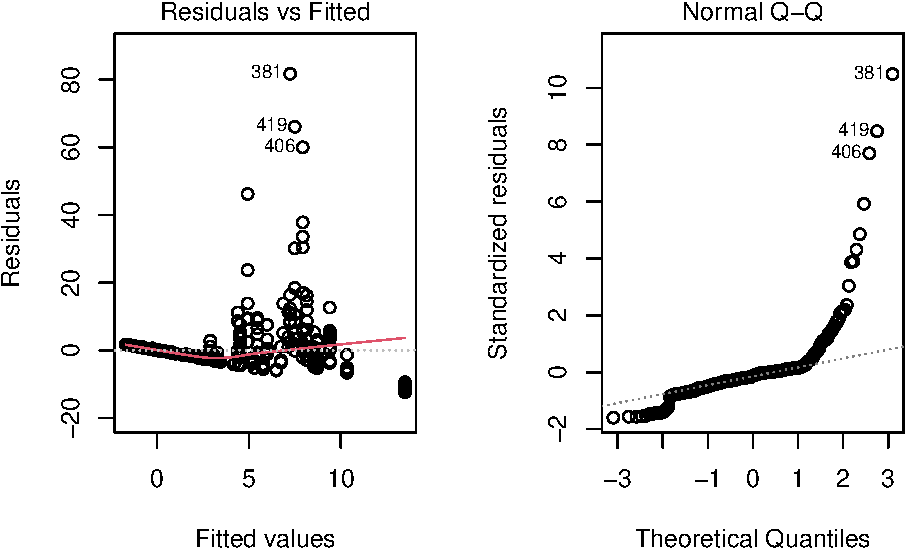
\includegraphics{Disha_Gandhi_Take_Home_Exam_PDF_files/figure-latex/unnamed-chunk-21-1.pdf}
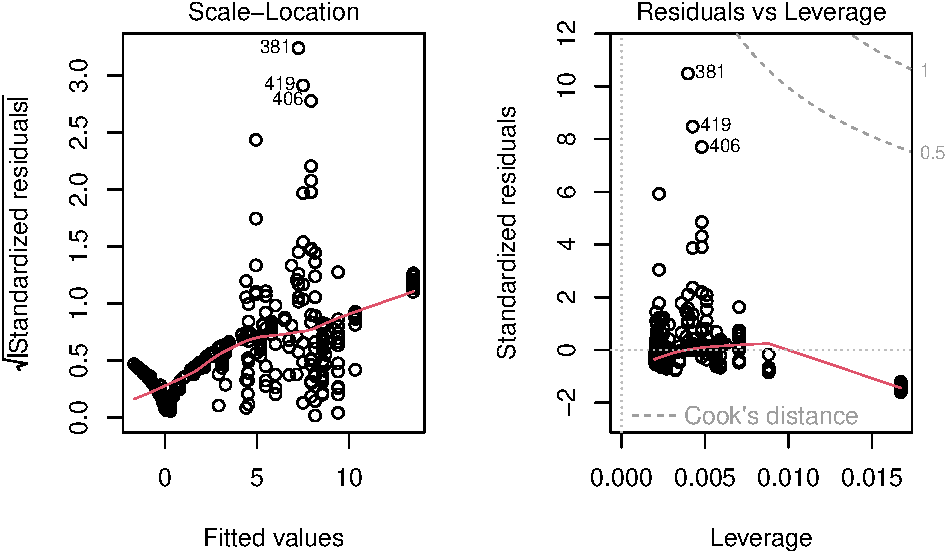
\includegraphics{Disha_Gandhi_Take_Home_Exam_PDF_files/figure-latex/unnamed-chunk-21-2.pdf}

\hypertarget{single-predictor---rm}{%
\subparagraph{\texorpdfstring{\textbf{Single Predictor -
RM}}{Single Predictor - RM}}\label{single-predictor---rm}}

\begin{verbatim}
## 
## Call:
## lm(formula = crim ~ rm)
## 
## Residuals:
##    Min     1Q Median     3Q    Max 
## -6.604 -3.952 -2.654  0.989 87.197 
## 
## Coefficients:
##             Estimate Std. Error t value Pr(>|t|)    
## (Intercept)   20.482      3.365   6.088 2.27e-09 ***
## rm            -2.684      0.532  -5.045 6.35e-07 ***
## ---
## Signif. codes:  0 '***' 0.001 '**' 0.01 '*' 0.05 '.' 0.1 ' ' 1
## 
## Residual standard error: 8.401 on 504 degrees of freedom
## Multiple R-squared:  0.04807,    Adjusted R-squared:  0.04618 
## F-statistic: 25.45 on 1 and 504 DF,  p-value: 6.347e-07
\end{verbatim}

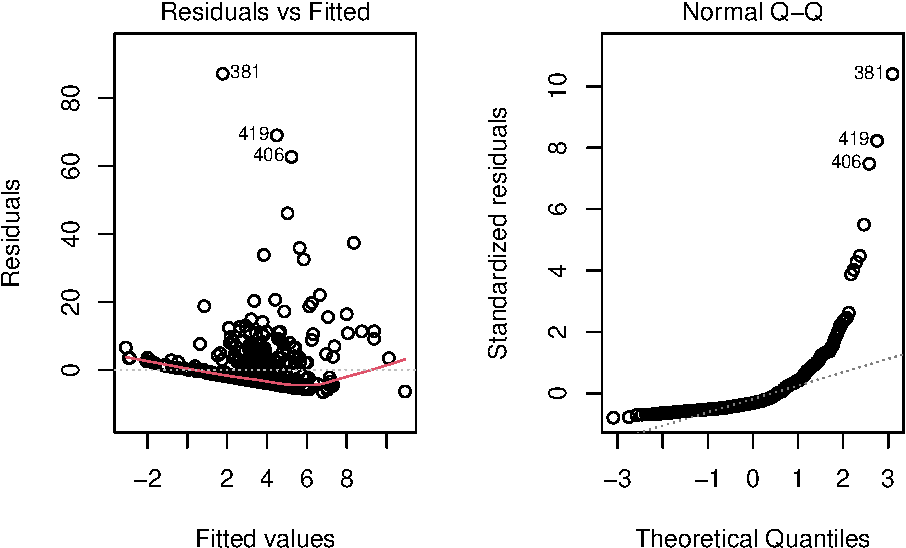
\includegraphics{Disha_Gandhi_Take_Home_Exam_PDF_files/figure-latex/unnamed-chunk-22-1.pdf}
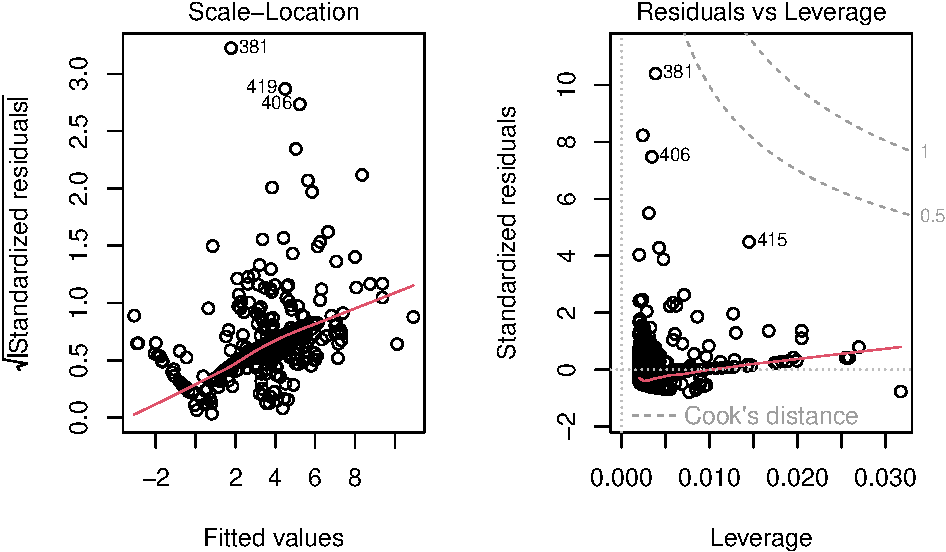
\includegraphics{Disha_Gandhi_Take_Home_Exam_PDF_files/figure-latex/unnamed-chunk-22-2.pdf}

\hypertarget{single-predictor---age}{%
\subparagraph{\texorpdfstring{\textbf{Single Predictor -
AGE}}{Single Predictor - AGE}}\label{single-predictor---age}}

\begin{verbatim}
## 
## Call:
## lm(formula = crim ~ age)
## 
## Residuals:
##    Min     1Q Median     3Q    Max 
## -6.789 -4.257 -1.230  1.527 82.849 
## 
## Coefficients:
##             Estimate Std. Error t value Pr(>|t|)    
## (Intercept) -3.77791    0.94398  -4.002 7.22e-05 ***
## age          0.10779    0.01274   8.463 2.85e-16 ***
## ---
## Signif. codes:  0 '***' 0.001 '**' 0.01 '*' 0.05 '.' 0.1 ' ' 1
## 
## Residual standard error: 8.057 on 504 degrees of freedom
## Multiple R-squared:  0.1244, Adjusted R-squared:  0.1227 
## F-statistic: 71.62 on 1 and 504 DF,  p-value: 2.855e-16
\end{verbatim}

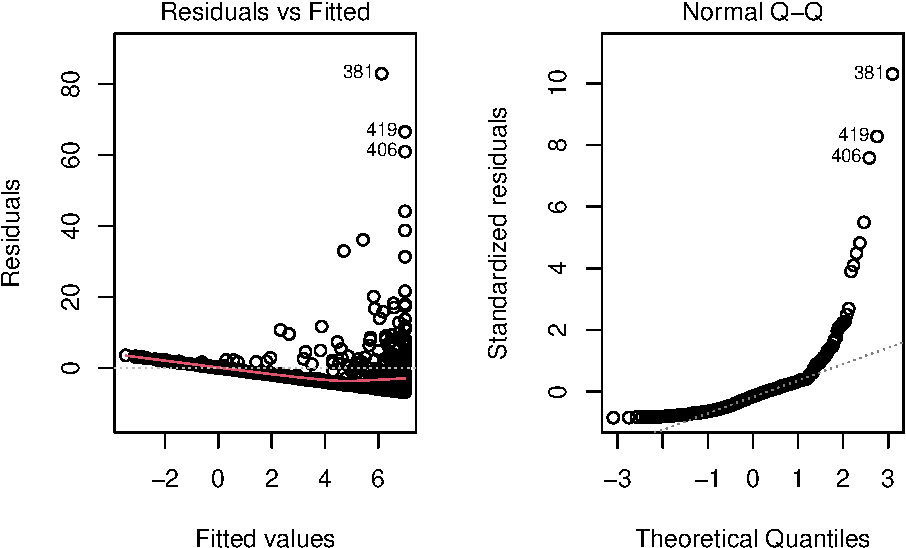
\includegraphics{Disha_Gandhi_Take_Home_Exam_PDF_files/figure-latex/unnamed-chunk-23-1.pdf}
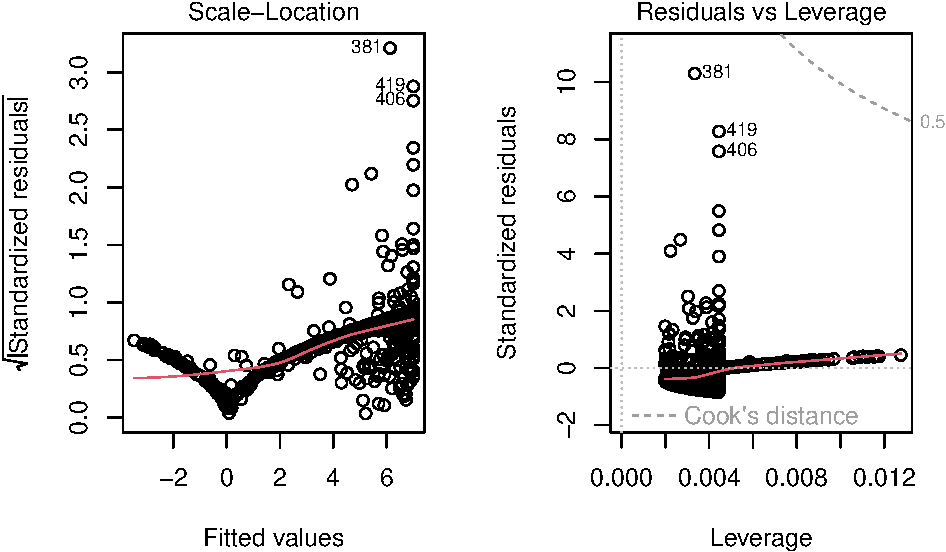
\includegraphics{Disha_Gandhi_Take_Home_Exam_PDF_files/figure-latex/unnamed-chunk-23-2.pdf}

\hypertarget{single-predictor---dis}{%
\subparagraph{\texorpdfstring{\textbf{Single Predictor -
DIS}}{Single Predictor - DIS}}\label{single-predictor---dis}}

\begin{verbatim}
## 
## Call:
## lm(formula = crim ~ dis)
## 
## Residuals:
##    Min     1Q Median     3Q    Max 
## -6.708 -4.134 -1.527  1.516 81.674 
## 
## Coefficients:
##             Estimate Std. Error t value Pr(>|t|)    
## (Intercept)   9.4993     0.7304  13.006   <2e-16 ***
## dis          -1.5509     0.1683  -9.213   <2e-16 ***
## ---
## Signif. codes:  0 '***' 0.001 '**' 0.01 '*' 0.05 '.' 0.1 ' ' 1
## 
## Residual standard error: 7.965 on 504 degrees of freedom
## Multiple R-squared:  0.1441, Adjusted R-squared:  0.1425 
## F-statistic: 84.89 on 1 and 504 DF,  p-value: < 2.2e-16
\end{verbatim}

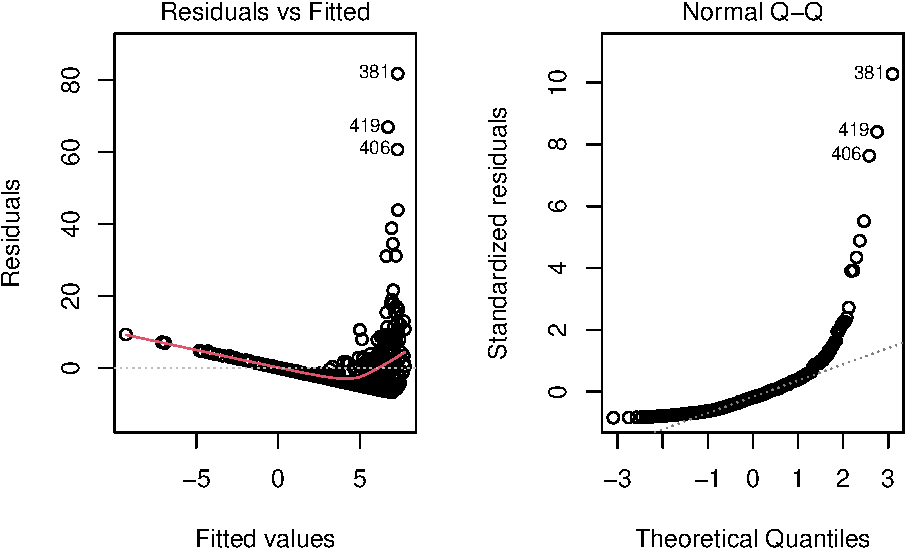
\includegraphics{Disha_Gandhi_Take_Home_Exam_PDF_files/figure-latex/unnamed-chunk-24-1.pdf}
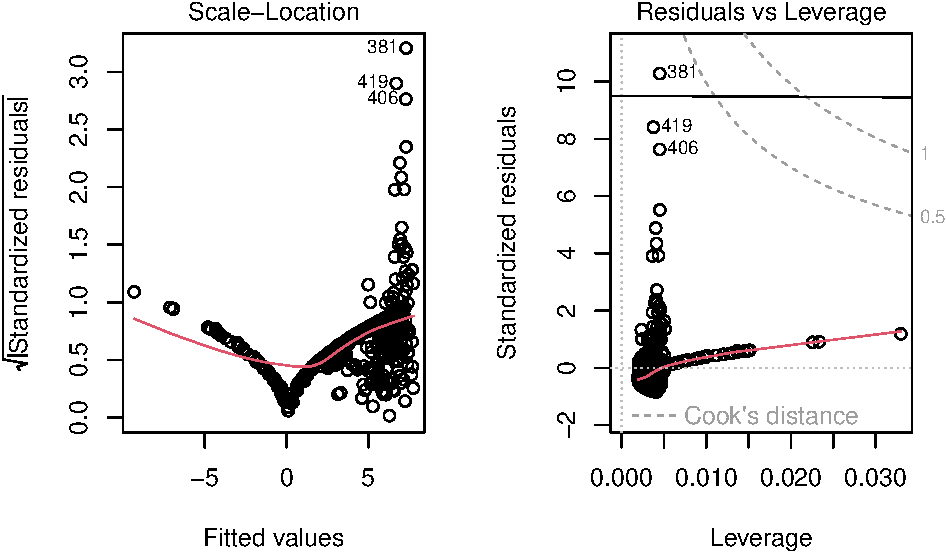
\includegraphics{Disha_Gandhi_Take_Home_Exam_PDF_files/figure-latex/unnamed-chunk-24-2.pdf}

\hypertarget{single-predictor---rad}{%
\subparagraph{\texorpdfstring{\textbf{Single Predictor -
RAD}}{Single Predictor - RAD}}\label{single-predictor---rad}}

\begin{verbatim}
## 
## Call:
## lm(formula = crim ~ rad)
## 
## Residuals:
##     Min      1Q  Median      3Q     Max 
## -10.164  -1.381  -0.141   0.660  76.433 
## 
## Coefficients:
##             Estimate Std. Error t value Pr(>|t|)    
## (Intercept) -2.28716    0.44348  -5.157 3.61e-07 ***
## rad          0.61791    0.03433  17.998  < 2e-16 ***
## ---
## Signif. codes:  0 '***' 0.001 '**' 0.01 '*' 0.05 '.' 0.1 ' ' 1
## 
## Residual standard error: 6.718 on 504 degrees of freedom
## Multiple R-squared:  0.3913, Adjusted R-squared:   0.39 
## F-statistic: 323.9 on 1 and 504 DF,  p-value: < 2.2e-16
\end{verbatim}

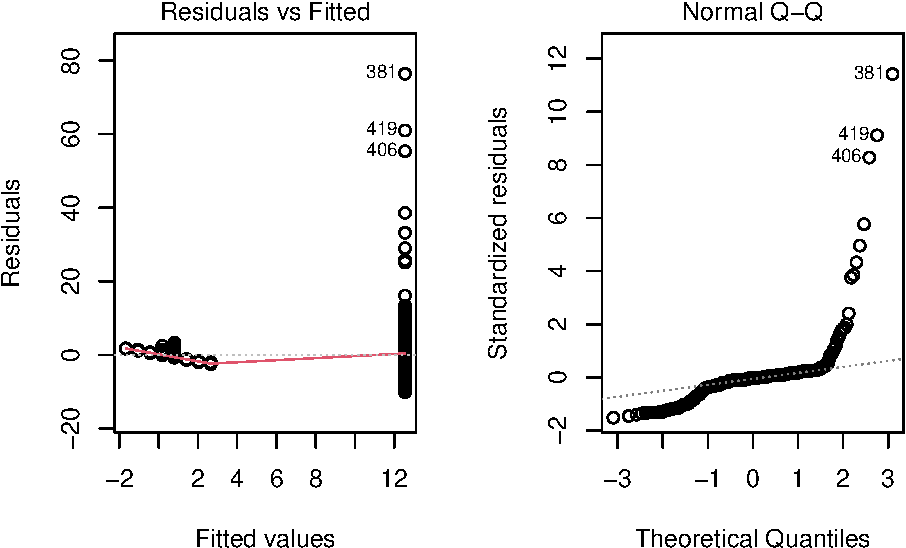
\includegraphics{Disha_Gandhi_Take_Home_Exam_PDF_files/figure-latex/unnamed-chunk-25-1.pdf}
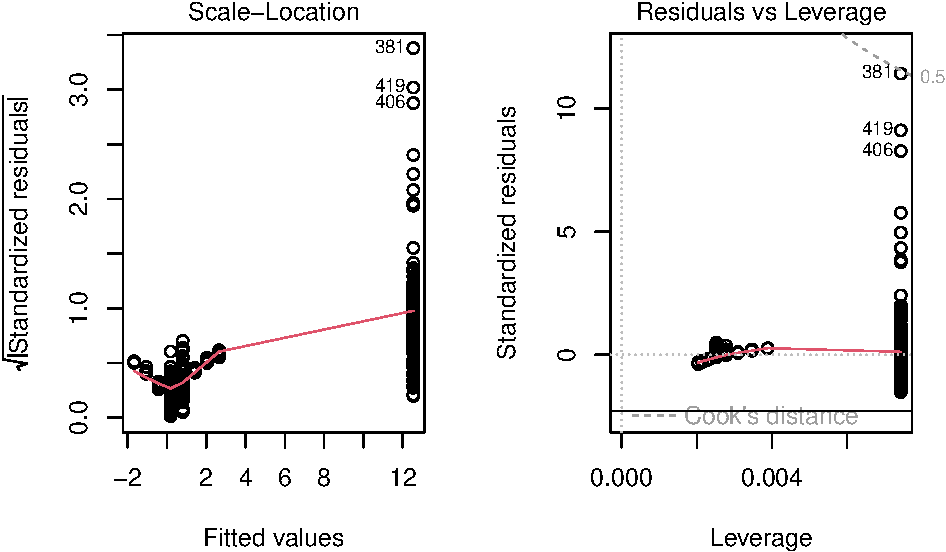
\includegraphics{Disha_Gandhi_Take_Home_Exam_PDF_files/figure-latex/unnamed-chunk-25-2.pdf}

\hypertarget{single-predictor---tax}{%
\subparagraph{\texorpdfstring{\textbf{Single Predictor -
TAX}}{Single Predictor - TAX}}\label{single-predictor---tax}}

\begin{verbatim}
## 
## Call:
## lm(formula = crim ~ tax)
## 
## Residuals:
##     Min      1Q  Median      3Q     Max 
## -12.513  -2.738  -0.194   1.065  77.696 
## 
## Coefficients:
##              Estimate Std. Error t value Pr(>|t|)    
## (Intercept) -8.528369   0.815809  -10.45   <2e-16 ***
## tax          0.029742   0.001847   16.10   <2e-16 ***
## ---
## Signif. codes:  0 '***' 0.001 '**' 0.01 '*' 0.05 '.' 0.1 ' ' 1
## 
## Residual standard error: 6.997 on 504 degrees of freedom
## Multiple R-squared:  0.3396, Adjusted R-squared:  0.3383 
## F-statistic: 259.2 on 1 and 504 DF,  p-value: < 2.2e-16
\end{verbatim}

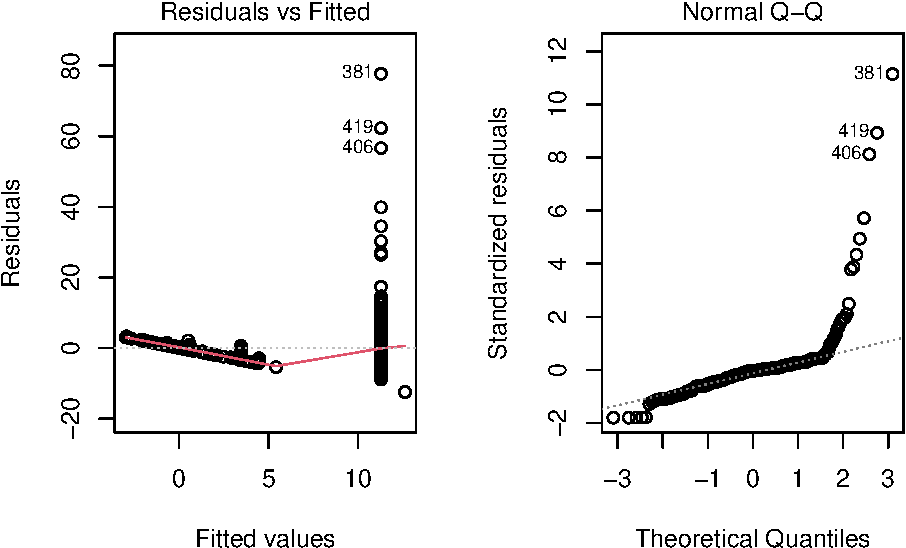
\includegraphics{Disha_Gandhi_Take_Home_Exam_PDF_files/figure-latex/unnamed-chunk-26-1.pdf}
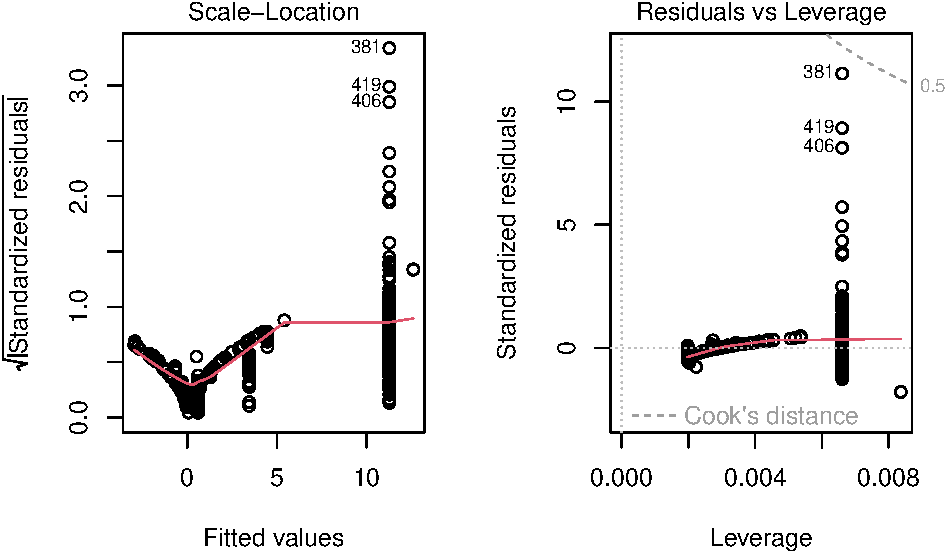
\includegraphics{Disha_Gandhi_Take_Home_Exam_PDF_files/figure-latex/unnamed-chunk-26-2.pdf}

\hypertarget{single-predictor---ptratio}{%
\subparagraph{\texorpdfstring{\textbf{Single Predictor -
PTRATIO}}{Single Predictor - PTRATIO}}\label{single-predictor---ptratio}}

\begin{verbatim}
## 
## Call:
## lm(formula = crim ~ ptratio)
## 
## Residuals:
##    Min     1Q Median     3Q    Max 
## -7.654 -3.985 -1.912  1.825 83.353 
## 
## Coefficients:
##             Estimate Std. Error t value Pr(>|t|)    
## (Intercept) -17.6469     3.1473  -5.607 3.40e-08 ***
## ptratio       1.1520     0.1694   6.801 2.94e-11 ***
## ---
## Signif. codes:  0 '***' 0.001 '**' 0.01 '*' 0.05 '.' 0.1 ' ' 1
## 
## Residual standard error: 8.24 on 504 degrees of freedom
## Multiple R-squared:  0.08407,    Adjusted R-squared:  0.08225 
## F-statistic: 46.26 on 1 and 504 DF,  p-value: 2.943e-11
\end{verbatim}

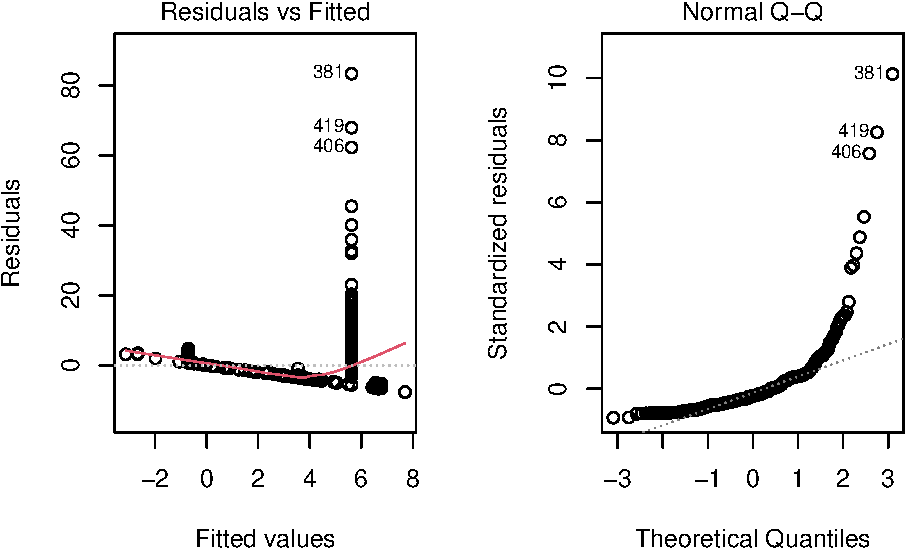
\includegraphics{Disha_Gandhi_Take_Home_Exam_PDF_files/figure-latex/unnamed-chunk-27-1.pdf}
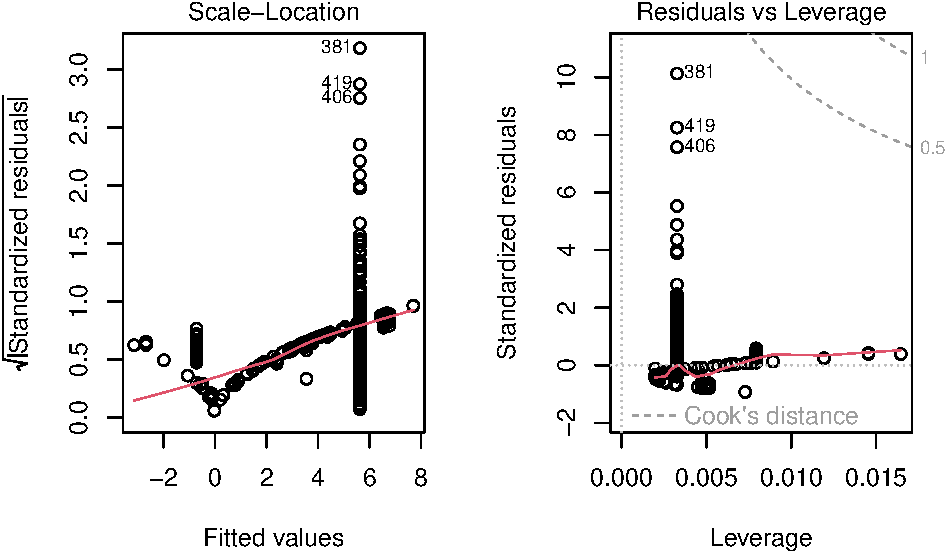
\includegraphics{Disha_Gandhi_Take_Home_Exam_PDF_files/figure-latex/unnamed-chunk-27-2.pdf}

\hypertarget{single-predictor---black}{%
\subparagraph{\texorpdfstring{\textbf{Single Predictor -
BLACK}}{Single Predictor - BLACK}}\label{single-predictor---black}}

\begin{verbatim}
## 
## Call:
## lm(formula = crim ~ black)
## 
## Residuals:
##     Min      1Q  Median      3Q     Max 
## -13.756  -2.299  -2.095  -1.296  86.822 
## 
## Coefficients:
##              Estimate Std. Error t value Pr(>|t|)    
## (Intercept) 16.553529   1.425903  11.609   <2e-16 ***
## black       -0.036280   0.003873  -9.367   <2e-16 ***
## ---
## Signif. codes:  0 '***' 0.001 '**' 0.01 '*' 0.05 '.' 0.1 ' ' 1
## 
## Residual standard error: 7.946 on 504 degrees of freedom
## Multiple R-squared:  0.1483, Adjusted R-squared:  0.1466 
## F-statistic: 87.74 on 1 and 504 DF,  p-value: < 2.2e-16
\end{verbatim}

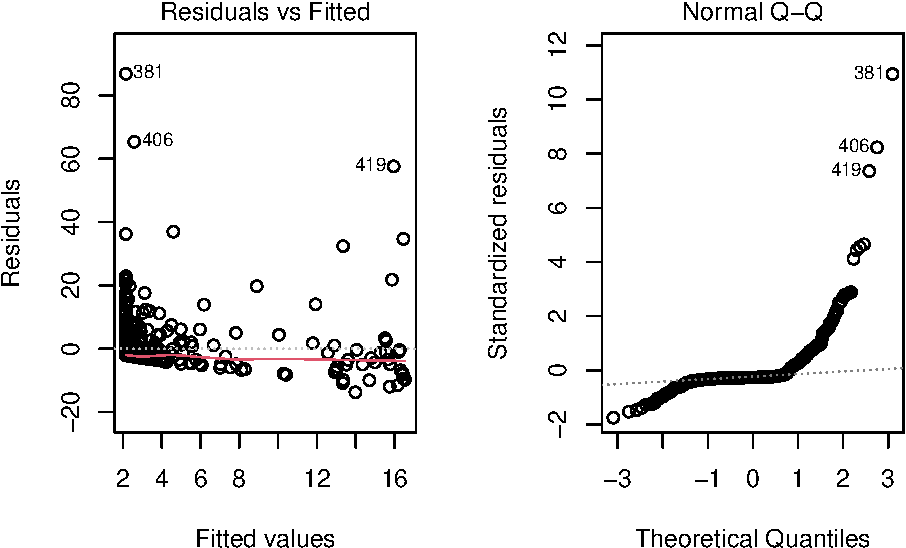
\includegraphics{Disha_Gandhi_Take_Home_Exam_PDF_files/figure-latex/unnamed-chunk-28-1.pdf}
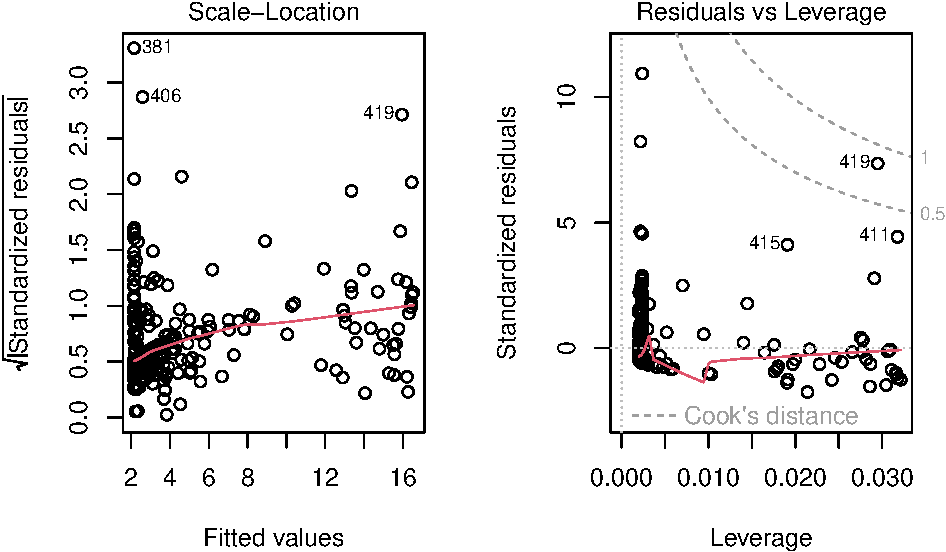
\includegraphics{Disha_Gandhi_Take_Home_Exam_PDF_files/figure-latex/unnamed-chunk-28-2.pdf}

\hypertarget{single-predictor---lstat}{%
\subparagraph{\texorpdfstring{\textbf{Single Predictor -
LSTAT}}{Single Predictor - LSTAT}}\label{single-predictor---lstat}}

\begin{verbatim}
## 
## Call:
## lm(formula = crim ~ lstat)
## 
## Residuals:
##     Min      1Q  Median      3Q     Max 
## -13.925  -2.822  -0.664   1.079  82.862 
## 
## Coefficients:
##             Estimate Std. Error t value Pr(>|t|)    
## (Intercept) -3.33054    0.69376  -4.801 2.09e-06 ***
## lstat        0.54880    0.04776  11.491  < 2e-16 ***
## ---
## Signif. codes:  0 '***' 0.001 '**' 0.01 '*' 0.05 '.' 0.1 ' ' 1
## 
## Residual standard error: 7.664 on 504 degrees of freedom
## Multiple R-squared:  0.2076, Adjusted R-squared:  0.206 
## F-statistic:   132 on 1 and 504 DF,  p-value: < 2.2e-16
\end{verbatim}

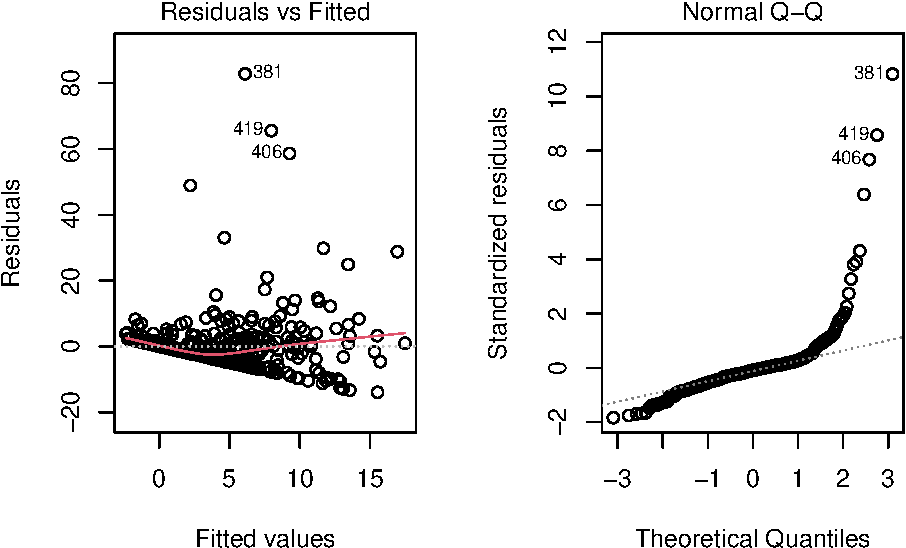
\includegraphics{Disha_Gandhi_Take_Home_Exam_PDF_files/figure-latex/unnamed-chunk-29-1.pdf}
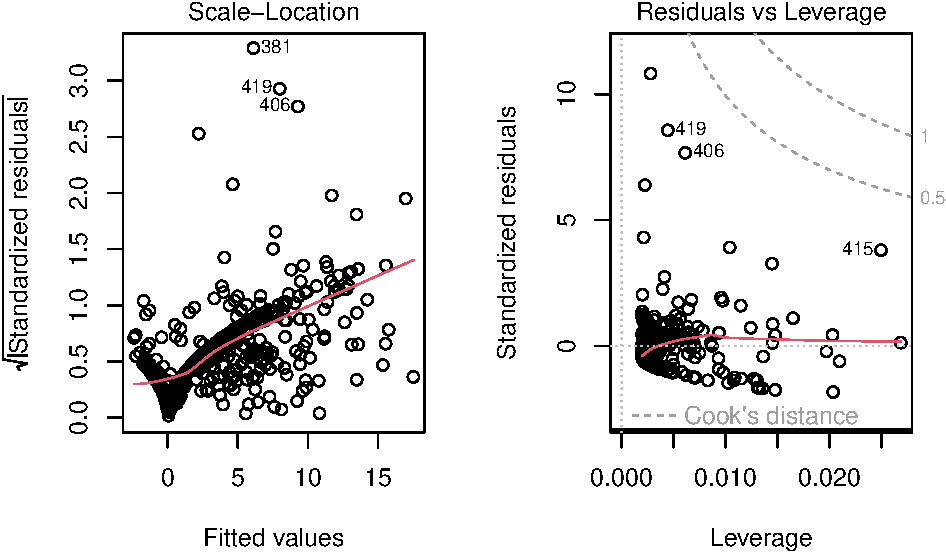
\includegraphics{Disha_Gandhi_Take_Home_Exam_PDF_files/figure-latex/unnamed-chunk-29-2.pdf}

\hypertarget{single-predictor---medv}{%
\subparagraph{\texorpdfstring{\textbf{Single Predictor -
MEDV}}{Single Predictor - MEDV}}\label{single-predictor---medv}}

\begin{verbatim}
## 
## Call:
## lm(formula = crim ~ medv)
## 
## Residuals:
##    Min     1Q Median     3Q    Max 
## -9.071 -4.022 -2.343  1.298 80.957 
## 
## Coefficients:
##             Estimate Std. Error t value Pr(>|t|)    
## (Intercept) 11.79654    0.93419   12.63   <2e-16 ***
## medv        -0.36316    0.03839   -9.46   <2e-16 ***
## ---
## Signif. codes:  0 '***' 0.001 '**' 0.01 '*' 0.05 '.' 0.1 ' ' 1
## 
## Residual standard error: 7.934 on 504 degrees of freedom
## Multiple R-squared:  0.1508, Adjusted R-squared:  0.1491 
## F-statistic: 89.49 on 1 and 504 DF,  p-value: < 2.2e-16
\end{verbatim}

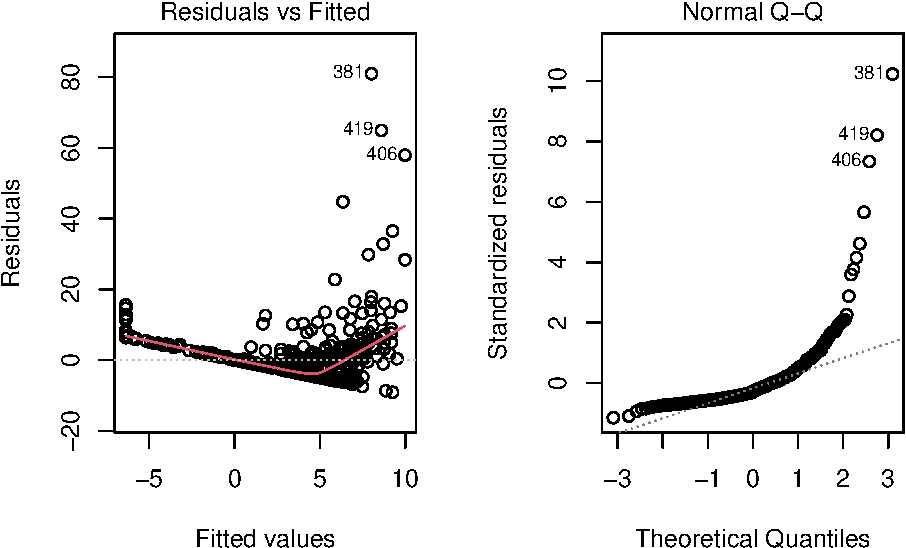
\includegraphics{Disha_Gandhi_Take_Home_Exam_PDF_files/figure-latex/unnamed-chunk-30-1.pdf}
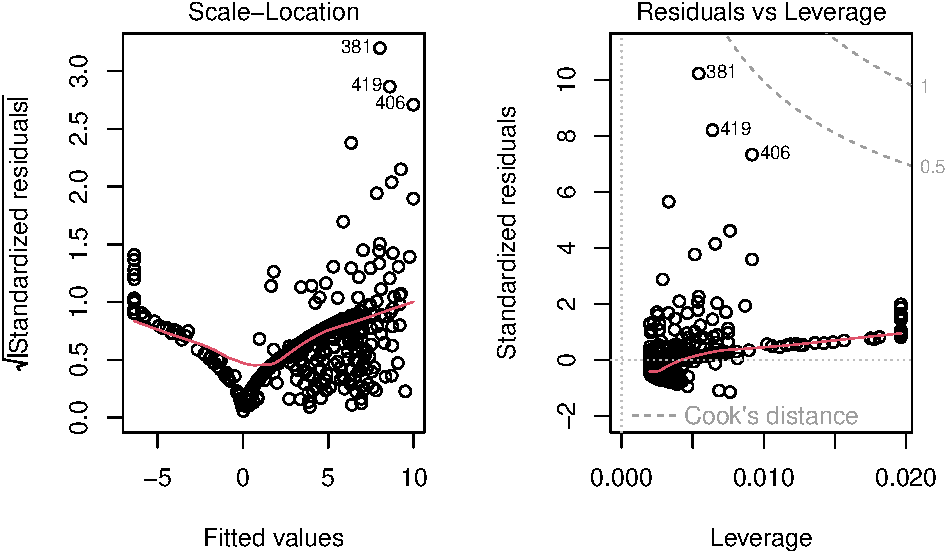
\includegraphics{Disha_Gandhi_Take_Home_Exam_PDF_files/figure-latex/unnamed-chunk-30-2.pdf}

\begin{itemize}
\item
  All the predictors except show a very small p value (\textless0.05)
  allowing us to conclude that all of them are statistically
  significant.
\item
  The residual vs predictor plot for all of them except chas have
  significant trend lines that are close to 0. This proves that we can
  rely on all of these fitted models except for chas, where we can't see
  any trend and the residual values are far from zero.
\item
  medv, dis, and age have quite a better linear regression line compared
  to other models showing they can be a good fit.
\end{itemize}

\hypertarget{part-b-1}{%
\paragraph{PART B}\label{part-b-1}}

\begin{verbatim}
## 
## Call:
## lm(formula = crim ~ ., data = Boston)
## 
## Residuals:
##    Min     1Q Median     3Q    Max 
## -9.924 -2.120 -0.353  1.019 75.051 
## 
## Coefficients:
##               Estimate Std. Error t value Pr(>|t|)    
## (Intercept)  17.033228   7.234903   2.354 0.018949 *  
## zn            0.044855   0.018734   2.394 0.017025 *  
## indus        -0.063855   0.083407  -0.766 0.444294    
## chas         -0.749134   1.180147  -0.635 0.525867    
## nox         -10.313535   5.275536  -1.955 0.051152 .  
## rm            0.430131   0.612830   0.702 0.483089    
## age           0.001452   0.017925   0.081 0.935488    
## dis          -0.987176   0.281817  -3.503 0.000502 ***
## rad           0.588209   0.088049   6.680 6.46e-11 ***
## tax          -0.003780   0.005156  -0.733 0.463793    
## ptratio      -0.271081   0.186450  -1.454 0.146611    
## black        -0.007538   0.003673  -2.052 0.040702 *  
## lstat         0.126211   0.075725   1.667 0.096208 .  
## medv         -0.198887   0.060516  -3.287 0.001087 ** 
## ---
## Signif. codes:  0 '***' 0.001 '**' 0.01 '*' 0.05 '.' 0.1 ' ' 1
## 
## Residual standard error: 6.439 on 492 degrees of freedom
## Multiple R-squared:  0.454,  Adjusted R-squared:  0.4396 
## F-statistic: 31.47 on 13 and 492 DF,  p-value: < 2.2e-16
\end{verbatim}

\begin{itemize}
\tightlist
\item
  We can see in the above summary that zn, dis, rad, black, and medv all
  have a p value less than 0.05 showing us that they are statistically
  significant to the above model and hence we can reject the null
  hypothesis for them.
\end{itemize}

\hypertarget{part-c-1}{%
\paragraph{PART C}\label{part-c-1}}

\begin{center}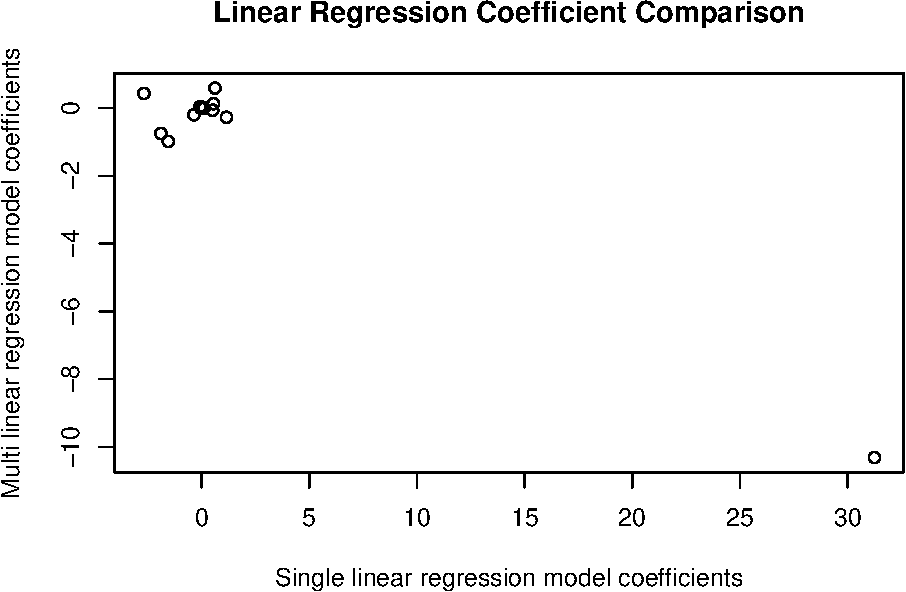
\includegraphics{Disha_Gandhi_Take_Home_Exam_PDF_files/figure-latex/unnamed-chunk-32-1} \end{center}

\begin{itemize}
\tightlist
\item
  All the features have almost similar coefficients in both cases other
  than nox for which the single linear regression model seems to have a
  very large positive coefficient whereas the multi linear model has a
  moderate negative coefficient.
\end{itemize}

\hypertarget{part-d-1}{%
\paragraph{PART D}\label{part-d-1}}

\hypertarget{single-non-linear-predictor---zn}{%
\subparagraph{\texorpdfstring{\textbf{Single Non Linear Predictor -
ZN}}{Single Non Linear Predictor - ZN}}\label{single-non-linear-predictor---zn}}

\begin{verbatim}
## 
## Call:
## lm(formula = crim ~ poly(zn, 3))
## 
## Residuals:
##    Min     1Q Median     3Q    Max 
## -4.821 -4.614 -1.294  0.473 84.130 
## 
## Coefficients:
##              Estimate Std. Error t value Pr(>|t|)    
## (Intercept)    3.6135     0.3722   9.709  < 2e-16 ***
## poly(zn, 3)1 -38.7498     8.3722  -4.628  4.7e-06 ***
## poly(zn, 3)2  23.9398     8.3722   2.859  0.00442 ** 
## poly(zn, 3)3 -10.0719     8.3722  -1.203  0.22954    
## ---
## Signif. codes:  0 '***' 0.001 '**' 0.01 '*' 0.05 '.' 0.1 ' ' 1
## 
## Residual standard error: 8.372 on 502 degrees of freedom
## Multiple R-squared:  0.05824,    Adjusted R-squared:  0.05261 
## F-statistic: 10.35 on 3 and 502 DF,  p-value: 1.281e-06
\end{verbatim}

\hypertarget{single-non-linear-predictor---indus}{%
\subparagraph{\texorpdfstring{\textbf{Single Non Linear Predictor -
INDUS}}{Single Non Linear Predictor - INDUS}}\label{single-non-linear-predictor---indus}}

\begin{verbatim}
## 
## Call:
## lm(formula = crim ~ poly(indus, 3))
## 
## Residuals:
##    Min     1Q Median     3Q    Max 
## -8.278 -2.514  0.054  0.764 79.713 
## 
## Coefficients:
##                 Estimate Std. Error t value Pr(>|t|)    
## (Intercept)        3.614      0.330  10.950  < 2e-16 ***
## poly(indus, 3)1   78.591      7.423  10.587  < 2e-16 ***
## poly(indus, 3)2  -24.395      7.423  -3.286  0.00109 ** 
## poly(indus, 3)3  -54.130      7.423  -7.292  1.2e-12 ***
## ---
## Signif. codes:  0 '***' 0.001 '**' 0.01 '*' 0.05 '.' 0.1 ' ' 1
## 
## Residual standard error: 7.423 on 502 degrees of freedom
## Multiple R-squared:  0.2597, Adjusted R-squared:  0.2552 
## F-statistic: 58.69 on 3 and 502 DF,  p-value: < 2.2e-16
\end{verbatim}

\hypertarget{single-non-linear-predictor---nox}{%
\subparagraph{\texorpdfstring{\textbf{Single Non Linear Predictor -
NOX}}{Single Non Linear Predictor - NOX}}\label{single-non-linear-predictor---nox}}

\begin{verbatim}
## 
## Call:
## lm(formula = crim ~ poly(nox, 3))
## 
## Residuals:
##    Min     1Q Median     3Q    Max 
## -9.110 -2.068 -0.255  0.739 78.302 
## 
## Coefficients:
##               Estimate Std. Error t value Pr(>|t|)    
## (Intercept)     3.6135     0.3216  11.237  < 2e-16 ***
## poly(nox, 3)1  81.3720     7.2336  11.249  < 2e-16 ***
## poly(nox, 3)2 -28.8286     7.2336  -3.985 7.74e-05 ***
## poly(nox, 3)3 -60.3619     7.2336  -8.345 6.96e-16 ***
## ---
## Signif. codes:  0 '***' 0.001 '**' 0.01 '*' 0.05 '.' 0.1 ' ' 1
## 
## Residual standard error: 7.234 on 502 degrees of freedom
## Multiple R-squared:  0.297,  Adjusted R-squared:  0.2928 
## F-statistic: 70.69 on 3 and 502 DF,  p-value: < 2.2e-16
\end{verbatim}

\hypertarget{single-non-linear-predictor---rm}{%
\subparagraph{\texorpdfstring{\textbf{Single Non Linear Predictor -
RM}}{Single Non Linear Predictor - RM}}\label{single-non-linear-predictor---rm}}

\begin{verbatim}
## 
## Call:
## lm(formula = crim ~ poly(rm, 3))
## 
## Residuals:
##     Min      1Q  Median      3Q     Max 
## -18.485  -3.468  -2.221  -0.015  87.219 
## 
## Coefficients:
##              Estimate Std. Error t value Pr(>|t|)    
## (Intercept)    3.6135     0.3703   9.758  < 2e-16 ***
## poly(rm, 3)1 -42.3794     8.3297  -5.088 5.13e-07 ***
## poly(rm, 3)2  26.5768     8.3297   3.191  0.00151 ** 
## poly(rm, 3)3  -5.5103     8.3297  -0.662  0.50858    
## ---
## Signif. codes:  0 '***' 0.001 '**' 0.01 '*' 0.05 '.' 0.1 ' ' 1
## 
## Residual standard error: 8.33 on 502 degrees of freedom
## Multiple R-squared:  0.06779,    Adjusted R-squared:  0.06222 
## F-statistic: 12.17 on 3 and 502 DF,  p-value: 1.067e-07
\end{verbatim}

\hypertarget{single-non-linear-predictor---age}{%
\subparagraph{\texorpdfstring{\textbf{Single Non Linear Predictor -
AGE}}{Single Non Linear Predictor - AGE}}\label{single-non-linear-predictor---age}}

\begin{verbatim}
## 
## Call:
## lm(formula = crim ~ poly(age, 3))
## 
## Residuals:
##    Min     1Q Median     3Q    Max 
## -9.762 -2.673 -0.516  0.019 82.842 
## 
## Coefficients:
##               Estimate Std. Error t value Pr(>|t|)    
## (Intercept)     3.6135     0.3485  10.368  < 2e-16 ***
## poly(age, 3)1  68.1820     7.8397   8.697  < 2e-16 ***
## poly(age, 3)2  37.4845     7.8397   4.781 2.29e-06 ***
## poly(age, 3)3  21.3532     7.8397   2.724  0.00668 ** 
## ---
## Signif. codes:  0 '***' 0.001 '**' 0.01 '*' 0.05 '.' 0.1 ' ' 1
## 
## Residual standard error: 7.84 on 502 degrees of freedom
## Multiple R-squared:  0.1742, Adjusted R-squared:  0.1693 
## F-statistic: 35.31 on 3 and 502 DF,  p-value: < 2.2e-16
\end{verbatim}

\hypertarget{single-non-linear-predictor---dis}{%
\subparagraph{\texorpdfstring{\textbf{Single Non Linear Predictor -
DIS}}{Single Non Linear Predictor - DIS}}\label{single-non-linear-predictor---dis}}

\begin{verbatim}
## 
## Call:
## lm(formula = crim ~ poly(dis, 3))
## 
## Residuals:
##     Min      1Q  Median      3Q     Max 
## -10.757  -2.588   0.031   1.267  76.378 
## 
## Coefficients:
##               Estimate Std. Error t value Pr(>|t|)    
## (Intercept)     3.6135     0.3259  11.087  < 2e-16 ***
## poly(dis, 3)1 -73.3886     7.3315 -10.010  < 2e-16 ***
## poly(dis, 3)2  56.3730     7.3315   7.689 7.87e-14 ***
## poly(dis, 3)3 -42.6219     7.3315  -5.814 1.09e-08 ***
## ---
## Signif. codes:  0 '***' 0.001 '**' 0.01 '*' 0.05 '.' 0.1 ' ' 1
## 
## Residual standard error: 7.331 on 502 degrees of freedom
## Multiple R-squared:  0.2778, Adjusted R-squared:  0.2735 
## F-statistic: 64.37 on 3 and 502 DF,  p-value: < 2.2e-16
\end{verbatim}

\hypertarget{single-non-linear-predictor---rad}{%
\subparagraph{\texorpdfstring{\textbf{Single Non Linear Predictor -
RAD}}{Single Non Linear Predictor - RAD}}\label{single-non-linear-predictor---rad}}

\begin{verbatim}
## 
## Call:
## lm(formula = crim ~ poly(rad, 3))
## 
## Residuals:
##     Min      1Q  Median      3Q     Max 
## -10.381  -0.412  -0.269   0.179  76.217 
## 
## Coefficients:
##               Estimate Std. Error t value Pr(>|t|)    
## (Intercept)     3.6135     0.2971  12.164  < 2e-16 ***
## poly(rad, 3)1 120.9074     6.6824  18.093  < 2e-16 ***
## poly(rad, 3)2  17.4923     6.6824   2.618  0.00912 ** 
## poly(rad, 3)3   4.6985     6.6824   0.703  0.48231    
## ---
## Signif. codes:  0 '***' 0.001 '**' 0.01 '*' 0.05 '.' 0.1 ' ' 1
## 
## Residual standard error: 6.682 on 502 degrees of freedom
## Multiple R-squared:    0.4,  Adjusted R-squared:  0.3965 
## F-statistic: 111.6 on 3 and 502 DF,  p-value: < 2.2e-16
\end{verbatim}

\hypertarget{single-non-linear-predictor---tax}{%
\subparagraph{\texorpdfstring{\textbf{Single Non Linear Predictor -
TAX}}{Single Non Linear Predictor - TAX}}\label{single-non-linear-predictor---tax}}

\begin{verbatim}
## 
## Call:
## lm(formula = crim ~ poly(tax, 3))
## 
## Residuals:
##     Min      1Q  Median      3Q     Max 
## -13.273  -1.389   0.046   0.536  76.950 
## 
## Coefficients:
##               Estimate Std. Error t value Pr(>|t|)    
## (Intercept)     3.6135     0.3047  11.860  < 2e-16 ***
## poly(tax, 3)1 112.6458     6.8537  16.436  < 2e-16 ***
## poly(tax, 3)2  32.0873     6.8537   4.682 3.67e-06 ***
## poly(tax, 3)3  -7.9968     6.8537  -1.167    0.244    
## ---
## Signif. codes:  0 '***' 0.001 '**' 0.01 '*' 0.05 '.' 0.1 ' ' 1
## 
## Residual standard error: 6.854 on 502 degrees of freedom
## Multiple R-squared:  0.3689, Adjusted R-squared:  0.3651 
## F-statistic:  97.8 on 3 and 502 DF,  p-value: < 2.2e-16
\end{verbatim}

\hypertarget{single-non-linear-predictor---ptratio}{%
\subparagraph{\texorpdfstring{\textbf{Single Non Linear Predictor -
PTRATIO}}{Single Non Linear Predictor - PTRATIO}}\label{single-non-linear-predictor---ptratio}}

\begin{verbatim}
## 
## Call:
## lm(formula = crim ~ poly(ptratio, 3))
## 
## Residuals:
##    Min     1Q Median     3Q    Max 
## -6.833 -4.146 -1.655  1.408 82.697 
## 
## Coefficients:
##                   Estimate Std. Error t value Pr(>|t|)    
## (Intercept)          3.614      0.361  10.008  < 2e-16 ***
## poly(ptratio, 3)1   56.045      8.122   6.901 1.57e-11 ***
## poly(ptratio, 3)2   24.775      8.122   3.050  0.00241 ** 
## poly(ptratio, 3)3  -22.280      8.122  -2.743  0.00630 ** 
## ---
## Signif. codes:  0 '***' 0.001 '**' 0.01 '*' 0.05 '.' 0.1 ' ' 1
## 
## Residual standard error: 8.122 on 502 degrees of freedom
## Multiple R-squared:  0.1138, Adjusted R-squared:  0.1085 
## F-statistic: 21.48 on 3 and 502 DF,  p-value: 4.171e-13
\end{verbatim}

\hypertarget{single-non-linear-predictor---black}{%
\subparagraph{\texorpdfstring{\textbf{Single Non Linear Predictor -
BLACK}}{Single Non Linear Predictor - BLACK}}\label{single-non-linear-predictor---black}}

\begin{verbatim}
## 
## Call:
## lm(formula = crim ~ poly(black, 3))
## 
## Residuals:
##     Min      1Q  Median      3Q     Max 
## -13.096  -2.343  -2.128  -1.439  86.790 
## 
## Coefficients:
##                 Estimate Std. Error t value Pr(>|t|)    
## (Intercept)       3.6135     0.3536  10.218   <2e-16 ***
## poly(black, 3)1 -74.4312     7.9546  -9.357   <2e-16 ***
## poly(black, 3)2   5.9264     7.9546   0.745    0.457    
## poly(black, 3)3  -4.8346     7.9546  -0.608    0.544    
## ---
## Signif. codes:  0 '***' 0.001 '**' 0.01 '*' 0.05 '.' 0.1 ' ' 1
## 
## Residual standard error: 7.955 on 502 degrees of freedom
## Multiple R-squared:  0.1498, Adjusted R-squared:  0.1448 
## F-statistic: 29.49 on 3 and 502 DF,  p-value: < 2.2e-16
\end{verbatim}

\hypertarget{single-non-linear-predictor---lstat}{%
\subparagraph{\texorpdfstring{\textbf{Single Non Linear Predictor -
LSTAT}}{Single Non Linear Predictor - LSTAT}}\label{single-non-linear-predictor---lstat}}

\begin{verbatim}
## 
## Call:
## lm(formula = crim ~ poly(lstat, 3))
## 
## Residuals:
##     Min      1Q  Median      3Q     Max 
## -15.234  -2.151  -0.486   0.066  83.353 
## 
## Coefficients:
##                 Estimate Std. Error t value Pr(>|t|)    
## (Intercept)       3.6135     0.3392  10.654   <2e-16 ***
## poly(lstat, 3)1  88.0697     7.6294  11.543   <2e-16 ***
## poly(lstat, 3)2  15.8882     7.6294   2.082   0.0378 *  
## poly(lstat, 3)3 -11.5740     7.6294  -1.517   0.1299    
## ---
## Signif. codes:  0 '***' 0.001 '**' 0.01 '*' 0.05 '.' 0.1 ' ' 1
## 
## Residual standard error: 7.629 on 502 degrees of freedom
## Multiple R-squared:  0.2179, Adjusted R-squared:  0.2133 
## F-statistic: 46.63 on 3 and 502 DF,  p-value: < 2.2e-16
\end{verbatim}

\hypertarget{single-non-linear-predictor---medv}{%
\subparagraph{\texorpdfstring{\textbf{Single Non Linear Predictor -
MEDV}}{Single Non Linear Predictor - MEDV}}\label{single-non-linear-predictor---medv}}

\begin{verbatim}
## 
## Call:
## lm(formula = crim ~ poly(medv, 3))
## 
## Residuals:
##     Min      1Q  Median      3Q     Max 
## -24.427  -1.976  -0.437   0.439  73.655 
## 
## Coefficients:
##                Estimate Std. Error t value Pr(>|t|)    
## (Intercept)       3.614      0.292  12.374  < 2e-16 ***
## poly(medv, 3)1  -75.058      6.569 -11.426  < 2e-16 ***
## poly(medv, 3)2   88.086      6.569  13.409  < 2e-16 ***
## poly(medv, 3)3  -48.033      6.569  -7.312 1.05e-12 ***
## ---
## Signif. codes:  0 '***' 0.001 '**' 0.01 '*' 0.05 '.' 0.1 ' ' 1
## 
## Residual standard error: 6.569 on 502 degrees of freedom
## Multiple R-squared:  0.4202, Adjusted R-squared:  0.4167 
## F-statistic: 121.3 on 3 and 502 DF,  p-value: < 2.2e-16
\end{verbatim}

\begin{itemize}
\tightlist
\item
  As we can see above,
\end{itemize}

-- zn has a lower p value i.e statistical significance for degrees 1 and
2.

-- indus has a lower p value i.e statistical significance for degrees 1,
2, and 3.

-- nox has a lower p value i.e statistical significance for degrees 1,
2, and 3.

-- rm has a lower p value i.e statistical significance for degrees 1 and
2.

-- age has a lower p value i.e statistical significance for degrees 1,
2, and 3.

-- dis has a lower p value i.e statistical significance for degrees 1,
2, and 3.

-- rad has a lower p value i.e statistical significance for degrees 1
and 2.

-- tax has a lower p value i.e statistical significance for degrees 1
and 2.

-- ptratio has a lower p value i.e statistical significance for degrees
1, 2, and 3.

-- black has a lower p value i.e statistical significance for degree 1
only.

-- lstat has a lower p value i.e statistical significance for degrees 1
and 2.

-- medv has a lower p value i.e statistical significance for degrees 1,
2, and 3.

\begin{itemize}
\tightlist
\item
  So there is evidence that we can fit all features into a non-linear
  model other than black and chas for which non linear relationship
  cannot exist as visible by the p value.
\end{itemize}

\hypertarget{chapter-6-question-9}{%
\subsection{CHAPTER 6 \textasciitilde{} QUESTION
9}\label{chapter-6-question-9}}

\hypertarget{part-a-2}{%
\paragraph{PART A}\label{part-a-2}}

The dataset is split into train and test as follows:

\begin{Shaded}
\begin{Highlighting}[]
\FunctionTok{attach}\NormalTok{(College)}

\DocumentationTok{\#\# 80\% of the sample size}
\NormalTok{train\_ind}\OtherTok{=}\FunctionTok{sample}\NormalTok{(}\FunctionTok{c}\NormalTok{(}\ConstantTok{TRUE}\NormalTok{ ,}\ConstantTok{FALSE}\NormalTok{), }\FunctionTok{nrow}\NormalTok{(College),}\AttributeTok{rep=}\ConstantTok{TRUE}\NormalTok{, }\AttributeTok{prob=}\FunctionTok{c}\NormalTok{(}\FloatTok{0.8}\NormalTok{,}\FloatTok{0.2}\NormalTok{))}

\NormalTok{train }\OtherTok{\textless{}{-}}\NormalTok{ College[train\_ind, ]}
\NormalTok{test }\OtherTok{\textless{}{-}}\NormalTok{ College[}\SpecialCharTok{{-}}\NormalTok{train\_ind, ]}
\end{Highlighting}
\end{Shaded}

\hypertarget{part-b-2}{%
\paragraph{PART B}\label{part-b-2}}

\begin{verbatim}
## [1] "The mean square test error on the linear model using least squares is 1067822.81531449"
\end{verbatim}

\hypertarget{part-c-2}{%
\paragraph{PART C}\label{part-c-2}}

\begin{verbatim}
## Loading required package: Matrix
\end{verbatim}

\begin{verbatim}
## Loaded glmnet 4.1-4
\end{verbatim}

\begin{verbatim}
## [1] "The best lambda for our ridge model is 0.01"
\end{verbatim}

\begin{verbatim}
## [1] "The mean square test error on the ridge model is 1067818.1872106"
\end{verbatim}

\hypertarget{part-d-2}{%
\paragraph{PART D}\label{part-d-2}}

\begin{verbatim}
## [1] "The best lambda for our lasso model is 0.01"
\end{verbatim}

\begin{verbatim}
## [1] "The mean square test error on the lasso model is 1067808.62956492"
\end{verbatim}

The list of coefficient values after fitting lasso model is

\begin{verbatim}
## 19 x 1 sparse Matrix of class "dgCMatrix"
##                        s1
## (Intercept) -471.39372052
## (Intercept)    .         
## PrivateYes  -491.04485137
## Accept         1.57033288
## Enroll        -0.75961467
## Top10perc     48.14698892
## Top25perc    -12.84690695
## F.Undergrad    0.04149116
## P.Undergrad    0.04438973
## Outstate      -0.08328388
## Room.Board     0.14943472
## Books          0.01532293
## Personal       0.02909954
## PhD           -8.39597537
## Terminal      -3.26800340
## S.F.Ratio     14.59298267
## perc.alumni   -0.04404771
## Expend         0.07712632
## Grad.Rate      8.28950241
\end{verbatim}

We can clearly see here that there are minimum two zero coefficients for
this dataset.

\hypertarget{part-e-1}{%
\paragraph{PART E}\label{part-e-1}}

\begin{verbatim}
## 
## Attaching package: 'pls'
\end{verbatim}

\begin{verbatim}
## The following object is masked from 'package:stats':
## 
##     loadings
\end{verbatim}

\begin{center}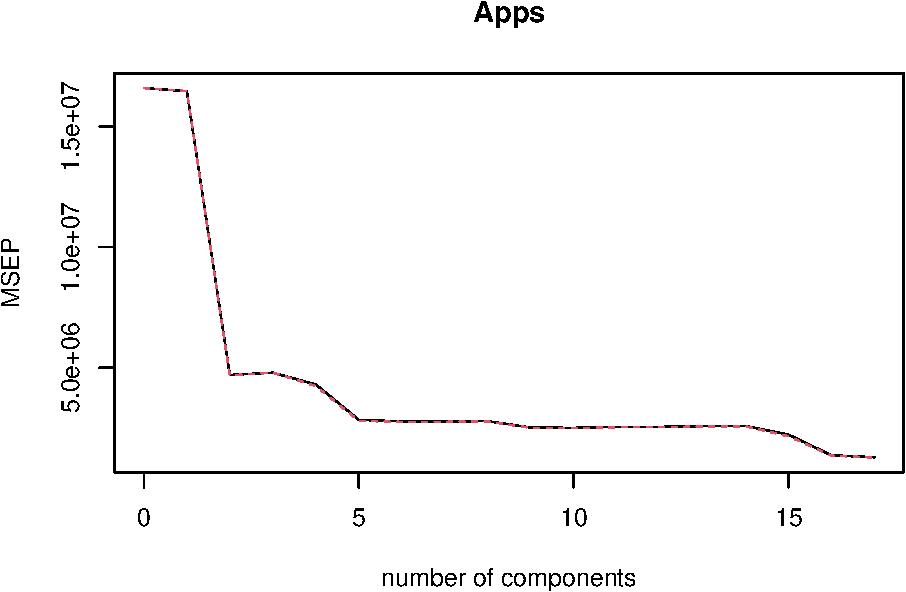
\includegraphics{Disha_Gandhi_Take_Home_Exam_PDF_files/figure-latex/unnamed-chunk-53-1} \end{center}

We can clearly see from the above plot that when the \textbf{number of
components is 10} we receive a considerable low CV score. So we now
predict on the test dataset using M=10.

\begin{verbatim}
## [1] "The mean square test error on the pcr model is 2103159.65327764"
\end{verbatim}

\hypertarget{part-f-1}{%
\paragraph{PART F}\label{part-f-1}}

\begin{center}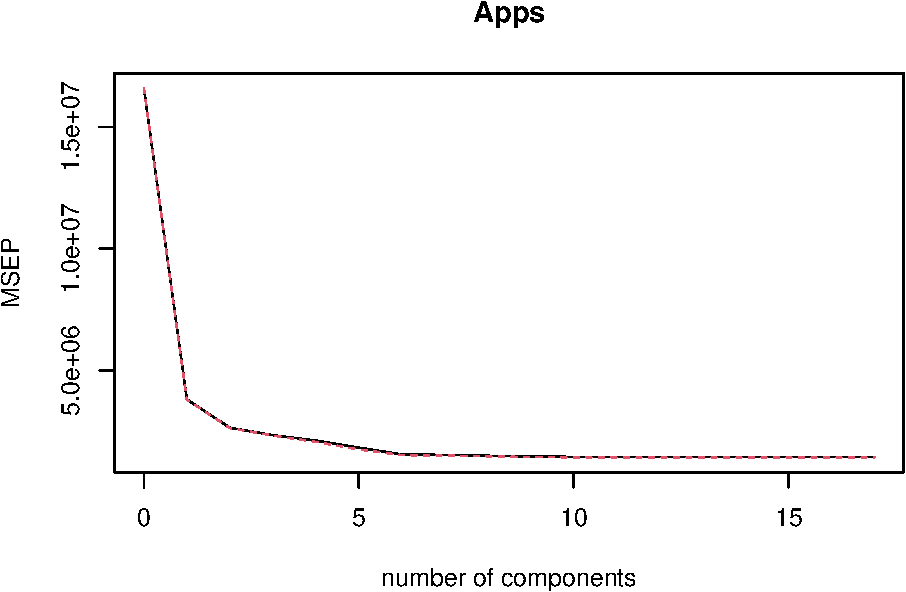
\includegraphics{Disha_Gandhi_Take_Home_Exam_PDF_files/figure-latex/unnamed-chunk-55-1} \end{center}

We can clearly see from the above plot that when the \textbf{number of
components is 10} we receive a considerable low CV score. So we now
predict on the test dataset using M=10.

\begin{verbatim}
## [1] "The mean square test error on the pls model is 1069554.36131769"
\end{verbatim}

\hypertarget{part-g-1}{%
\paragraph{\texorpdfstring{{PART G}}{PART G}}\label{part-g-1}}

\begin{center}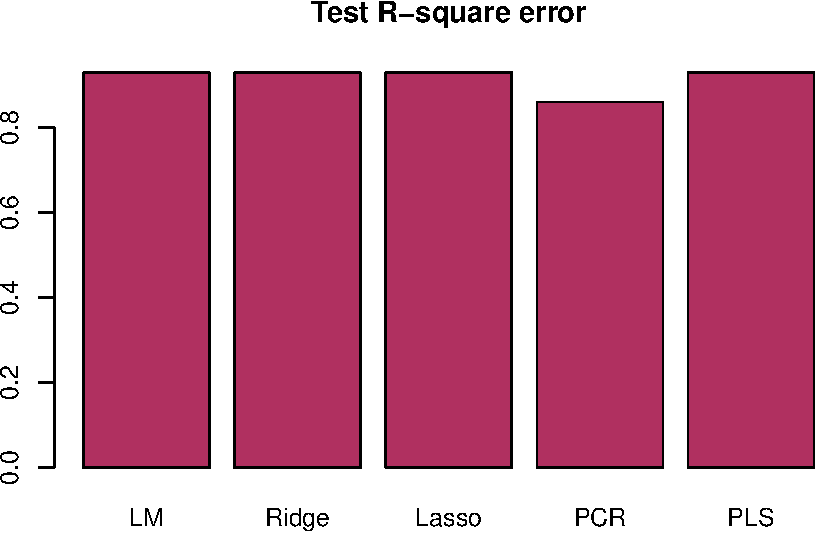
\includegraphics{Disha_Gandhi_Take_Home_Exam_PDF_files/figure-latex/unnamed-chunk-57-1} \end{center}

\begin{itemize}
\item
  This plot shows that accuracy for all models is about 0.9 but PCR has
  a relatively lower accuracy. So we can predict all model except PCR
  has a high accuracy.
\item
  Linear Regression, Ridge, and Lasso have comparable test errors. But
  PCR has a significantly high test error rate when compared to other
  models.
\item
  PLS shows the test error rate in the same range as linear regression,
  Lasso, and Ridge just a little less and hence slightly better in this
  dataset.
\end{itemize}

\hypertarget{chapter-6-question-11}{%
\subsection{CHAPTER 6 \textasciitilde{} QUESTION
11}\label{chapter-6-question-11}}

\hypertarget{part-a-3}{%
\paragraph{\texorpdfstring{{PART A}}{PART A}}\label{part-a-3}}

\hypertarget{best-subset-selection-model}{%
\subparagraph{\texorpdfstring{\textbf{Best Subset Selection
Model}}{Best Subset Selection Model}}\label{best-subset-selection-model}}

\begin{verbatim}
## Subset selection object
## Call: regsubsets.formula(crim ~ ., Boston, nvmax = 13)
## 13 Variables  (and intercept)
##         Forced in Forced out
## zn          FALSE      FALSE
## indus       FALSE      FALSE
## chas        FALSE      FALSE
## nox         FALSE      FALSE
## rm          FALSE      FALSE
## age         FALSE      FALSE
## dis         FALSE      FALSE
## rad         FALSE      FALSE
## tax         FALSE      FALSE
## ptratio     FALSE      FALSE
## black       FALSE      FALSE
## lstat       FALSE      FALSE
## medv        FALSE      FALSE
## 1 subsets of each size up to 13
## Selection Algorithm: exhaustive
##           zn  indus chas nox rm  age dis rad tax ptratio black lstat medv
## 1  ( 1 )  " " " "   " "  " " " " " " " " "*" " " " "     " "   " "   " " 
## 2  ( 1 )  " " " "   " "  " " " " " " " " "*" " " " "     " "   "*"   " " 
## 3  ( 1 )  " " " "   " "  " " " " " " " " "*" " " " "     "*"   "*"   " " 
## 4  ( 1 )  "*" " "   " "  " " " " " " "*" "*" " " " "     " "   " "   "*" 
## 5  ( 1 )  "*" " "   " "  " " " " " " "*" "*" " " " "     "*"   " "   "*" 
## 6  ( 1 )  "*" " "   " "  "*" " " " " "*" "*" " " " "     "*"   " "   "*" 
## 7  ( 1 )  "*" " "   " "  "*" " " " " "*" "*" " " "*"     "*"   " "   "*" 
## 8  ( 1 )  "*" " "   " "  "*" " " " " "*" "*" " " "*"     "*"   "*"   "*" 
## 9  ( 1 )  "*" "*"   " "  "*" " " " " "*" "*" " " "*"     "*"   "*"   "*" 
## 10  ( 1 ) "*" "*"   " "  "*" "*" " " "*" "*" " " "*"     "*"   "*"   "*" 
## 11  ( 1 ) "*" "*"   " "  "*" "*" " " "*" "*" "*" "*"     "*"   "*"   "*" 
## 12  ( 1 ) "*" "*"   "*"  "*" "*" " " "*" "*" "*" "*"     "*"   "*"   "*" 
## 13  ( 1 ) "*" "*"   "*"  "*" "*" "*" "*" "*" "*" "*"     "*"   "*"   "*"
\end{verbatim}

\begin{center}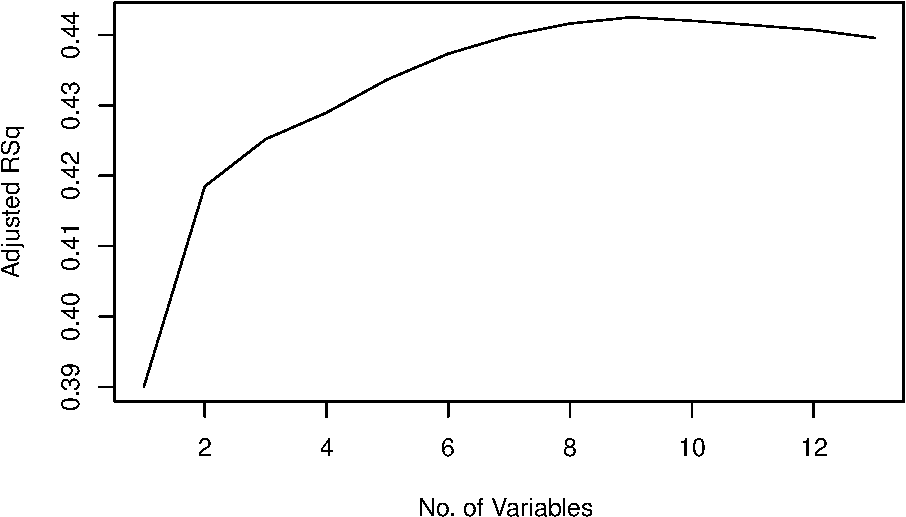
\includegraphics{Disha_Gandhi_Take_Home_Exam_PDF_files/figure-latex/unnamed-chunk-58-1} \end{center}

\begin{verbatim}
## [1] 9
\end{verbatim}

\begin{verbatim}
## [1] "The ideal number of features as suggested by Best Subset Selection is 9"
\end{verbatim}

\begin{verbatim}
## [1] "And the corresponding adjusted r square error for the test dataset is 0.442505260718671"
\end{verbatim}

The list of those 9 features as suggested above is:

\begin{verbatim}
##   (Intercept)            zn         indus           nox           dis 
##  19.124636156   0.042788127  -0.099385948 -10.466490364  -1.002597606 
##           rad       ptratio         black         lstat          medv 
##   0.539503547  -0.270835584  -0.008003761   0.117805932  -0.180593877
\end{verbatim}

\hypertarget{linear-regression-model}{%
\subparagraph{\texorpdfstring{\textbf{Linear Regression
Model}}{Linear Regression Model}}\label{linear-regression-model}}

What I then did was fit a multi linear regression model on those 9
features and check the RMSE.

\begin{verbatim}
## 
## Call:
## lm(formula = crim ~ zn + nox + rm + dis + rad + tax + ptratio + 
##     black + medv)
## 
## Residuals:
##     Min      1Q  Median      3Q     Max 
## -10.087  -1.981  -0.486   0.946  74.771 
## 
## Coefficients:
##               Estimate Std. Error t value Pr(>|t|)    
## (Intercept)  22.292764   6.620265   3.367 0.000818 ***
## zn            0.049143   0.018415   2.669 0.007866 ** 
## nox         -10.994625   4.849178  -2.267 0.023800 *  
## rm            0.234791   0.579258   0.405 0.685409    
## dis          -1.061451   0.257214  -4.127 4.32e-05 ***
## rad           0.621492   0.083172   7.472 3.59e-13 ***
## tax          -0.005657   0.004622  -1.224 0.221574    
## ptratio      -0.307299   0.183800  -1.672 0.095172 .  
## black        -0.007929   0.003654  -2.170 0.030500 *  
## medv         -0.253518   0.053032  -4.780 2.31e-06 ***
## ---
## Signif. codes:  0 '***' 0.001 '**' 0.01 '*' 0.05 '.' 0.1 ' ' 1
## 
## Residual standard error: 6.439 on 496 degrees of freedom
## Multiple R-squared:  0.4496, Adjusted R-squared:  0.4396 
## F-statistic: 45.01 on 9 and 496 DF,  p-value: < 2.2e-16
\end{verbatim}

We observed an RMSE of \textbf{6.439}, which is lower than best subset
selection.

\hypertarget{ridge-regression}{%
\subparagraph{\texorpdfstring{\textbf{Ridge
Regression}}{Ridge Regression}}\label{ridge-regression}}

\begin{center}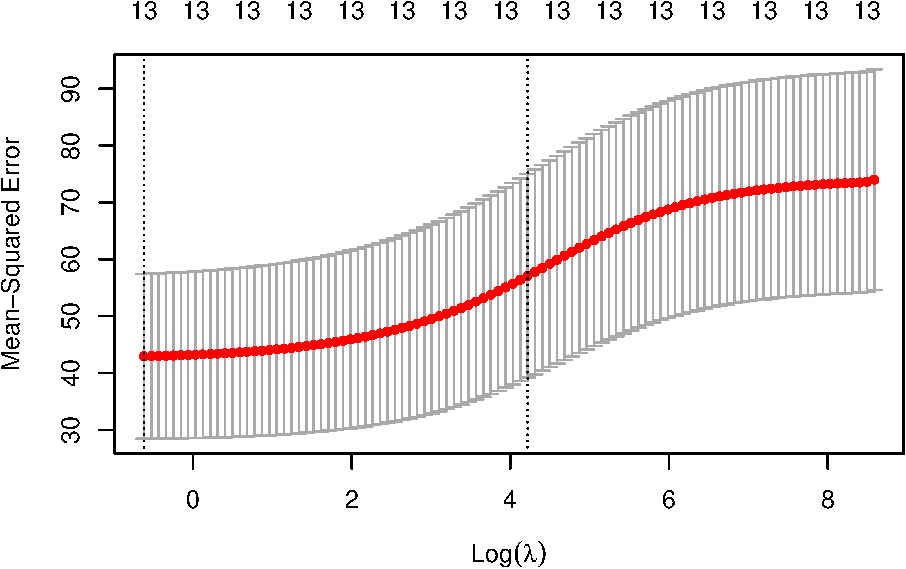
\includegraphics{Disha_Gandhi_Take_Home_Exam_PDF_files/figure-latex/unnamed-chunk-62-1} \end{center}

\begin{verbatim}
## [1] "The root mean square test error on the ridge model is 7.55549865637999"
\end{verbatim}

\hypertarget{lasso-regression}{%
\subparagraph{\texorpdfstring{\textbf{Lasso
Regression}}{Lasso Regression}}\label{lasso-regression}}

\begin{center}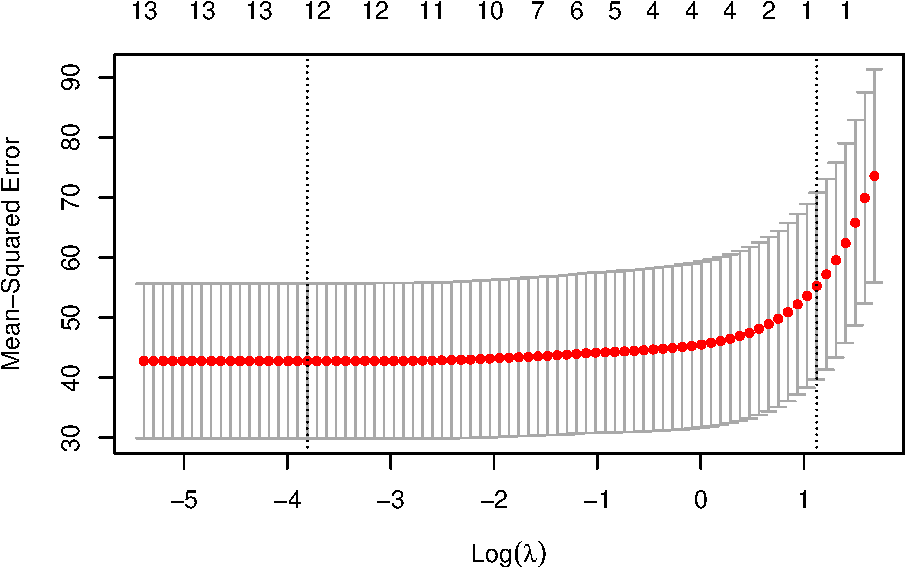
\includegraphics{Disha_Gandhi_Take_Home_Exam_PDF_files/figure-latex/unnamed-chunk-64-1} \end{center}

\begin{verbatim}
## [1] "The root mean square test error on the lasso model is 7.43206681747073"
\end{verbatim}

\hypertarget{principal-components-regression}{%
\subparagraph{\texorpdfstring{\textbf{Principal Components
Regression}}{Principal Components Regression}}\label{principal-components-regression}}

\begin{verbatim}
## Data:    X dimension: 506 13 
##  Y dimension: 506 1
## Fit method: svdpc
## Number of components considered: 13
## 
## VALIDATION: RMSEP
## Cross-validated using 10 random segments.
##        (Intercept)  1 comps  2 comps  3 comps  4 comps  5 comps  6 comps
## CV            8.61    7.226    7.223    6.803    6.781    6.799    6.848
## adjCV         8.61    7.222    7.219    6.796    6.773    6.792    6.838
##        7 comps  8 comps  9 comps  10 comps  11 comps  12 comps  13 comps
## CV       6.842    6.705    6.734     6.717     6.716     6.682     6.606
## adjCV    6.832    6.694    6.721     6.705     6.704     6.668     6.593
## 
## TRAINING: % variance explained
##       1 comps  2 comps  3 comps  4 comps  5 comps  6 comps  7 comps  8 comps
## X       47.70    60.36    69.67    76.45    82.99    88.00    91.14    93.45
## crim    30.69    30.87    39.27    39.61    39.61    39.86    40.14    42.47
##       9 comps  10 comps  11 comps  12 comps  13 comps
## X       95.40     97.04     98.46     99.52     100.0
## crim    42.55     42.78     43.04     44.13      45.4
\end{verbatim}

We can here clearly see that 13 component pcr model has a cv error of
\textbf{6.606}

\begin{itemize}
\tightlist
\item
  To summarize we can observe that 9 component linear regression
  followed by 9 component best subset model followed by 13 component pcr
  have the cv errors in this order respectively. Hence the linear
  regression model seems to be a good fit
\end{itemize}

\hypertarget{part-b-3}{%
\paragraph{\texorpdfstring{{PART B}}{PART B}}\label{part-b-3}}

\begin{itemize}
\item
  After looking at various models that we fit above, we can see that the
  lowest cv error is observed for the 9 component Linear Regression
  Model. The cv error for 13 component PCR is only a little higher than
  this.
\item
  So my proposal would be to fit a best subset model to find out the
  ideal features and then use those features to fit a linear regression
  model.
\end{itemize}

\hypertarget{part-c-3}{%
\paragraph{\texorpdfstring{{PART C}}{PART C}}\label{part-c-3}}

\begin{itemize}
\tightlist
\item
  My chosen model involves only 9 features as listed above, since the
  test RMSE is lowest when only these 9 features are fit. Upon fitting a
  Linear model with all features, the RMSE was slightly higher.
\end{itemize}

\hypertarget{chapter-8-question-8}{%
\subsection{CHAPTER 8 \textasciitilde{} QUESTION
8}\label{chapter-8-question-8}}

\hypertarget{part-a-4}{%
\paragraph{\texorpdfstring{{PART A}}{PART A}}\label{part-a-4}}

The dataset is split into train and test as follows:

\begin{Shaded}
\begin{Highlighting}[]
\FunctionTok{library}\NormalTok{(ISLR)}
\FunctionTok{attach}\NormalTok{(Carseats)}
 
\DocumentationTok{\#\# 80\% of the sample size}
\NormalTok{smp\_size }\OtherTok{\textless{}{-}} \FunctionTok{floor}\NormalTok{(}\FloatTok{0.80} \SpecialCharTok{*} \FunctionTok{nrow}\NormalTok{(Carseats))}
 
\NormalTok{train\_ind }\OtherTok{\textless{}{-}} \FunctionTok{sample}\NormalTok{(}\FunctionTok{seq\_len}\NormalTok{(}\FunctionTok{nrow}\NormalTok{(Carseats)), }\AttributeTok{size =}\NormalTok{ smp\_size)}
 
\NormalTok{train }\OtherTok{\textless{}{-}}\NormalTok{ Carseats[train\_ind, ]}
\NormalTok{test }\OtherTok{\textless{}{-}}\NormalTok{ Carseats[}\SpecialCharTok{{-}}\NormalTok{train\_ind, ]}
\end{Highlighting}
\end{Shaded}

\hypertarget{part-b-4}{%
\paragraph{\texorpdfstring{{PART B}}{PART B}}\label{part-b-4}}

\begin{verbatim}
## 
## Regression tree:
## tree(formula = Sales ~ ., data = train)
## Variables actually used in tree construction:
## [1] "ShelveLoc"   "Price"       "CompPrice"   "Income"      "Age"        
## [6] "Advertising"
## Number of terminal nodes:  18 
## Residual mean deviance:  2.578 = 778.4 / 302 
## Distribution of residuals:
##    Min. 1st Qu.  Median    Mean 3rd Qu.    Max. 
## -4.0620 -1.0600 -0.0272  0.0000  1.0340  4.9080
\end{verbatim}

\begin{center}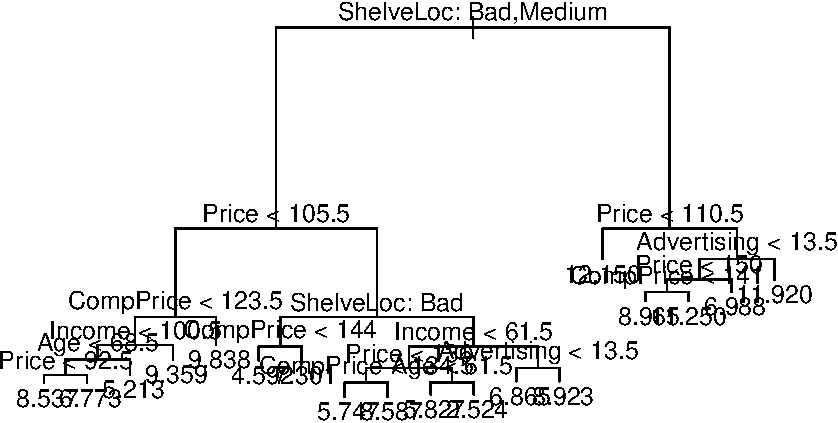
\includegraphics{Disha_Gandhi_Take_Home_Exam_PDF_files/figure-latex/unnamed-chunk-69-1} \end{center}

\begin{verbatim}
## [1] "The  mean square test error on the regression tree is 4.15262426048523"
\end{verbatim}

\begin{itemize}
\item
  The tree here shows that ShelveLoc and Price are the two important
  features for splitting the tree.
\item
  Even the residual deviance is not so high implying the tree was fit
  good on the training dataset.
\end{itemize}

\hypertarget{part-c-4}{%
\paragraph{\texorpdfstring{{PART C}}{PART C}}\label{part-c-4}}

\begin{center}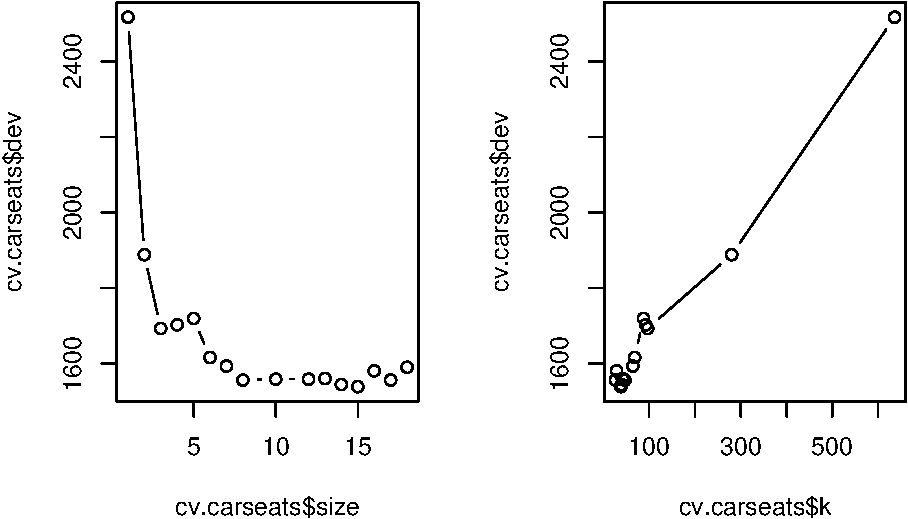
\includegraphics{Disha_Gandhi_Take_Home_Exam_PDF_files/figure-latex/unnamed-chunk-71-1} \end{center}

Since we get the lowest value of the size variable at 10 components, we
will fit the pruned tree with 10 features.

\begin{center}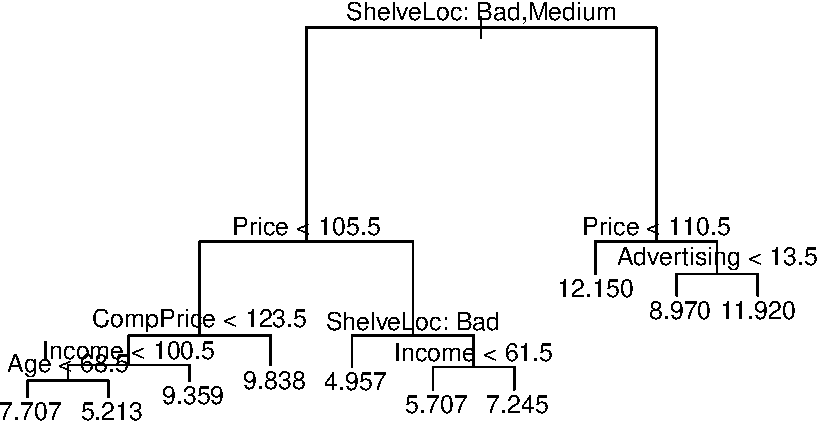
\includegraphics{Disha_Gandhi_Take_Home_Exam_PDF_files/figure-latex/unnamed-chunk-72-1} \end{center}

\begin{verbatim}
## [1] "The  mean square test error on the pruned regression tree is 4.17694642471046"
\end{verbatim}

\begin{itemize}
\item
  We can see over here that the mean square test error just increased
  after prunning, telling us that the vanilla regression tree is a
  better version for our dataset than pruned one.
\item
  ALso, even after prunning the tree we get the same two features,
  ShelveLoc and Price as the top two features for the best split of the
  tree.
\end{itemize}

\hypertarget{part-d-3}{%
\paragraph{\texorpdfstring{{PART D}}{PART D}}\label{part-d-3}}

\begin{verbatim}
## randomForest 4.7-1.1
\end{verbatim}

\begin{verbatim}
## Type rfNews() to see new features/changes/bug fixes.
\end{verbatim}

\begin{verbatim}
## [1] "The  mean square test error in bagging is 2.18869707426279"
\end{verbatim}

\begin{verbatim}
##                %IncMSE IncNodePurity
## CompPrice   35.3935974    292.945903
## Income       9.6864287    132.850808
## Advertising 21.8796713    202.131987
## Population  -0.7539982     90.173094
## Price       71.4861471    675.405214
## ShelveLoc   78.6727173    750.633543
## Age         19.7410078    212.870856
## Education    4.7078674     75.346672
## Urban        0.3655543     14.877175
## US           0.0981082      8.576228
\end{verbatim}

\begin{center}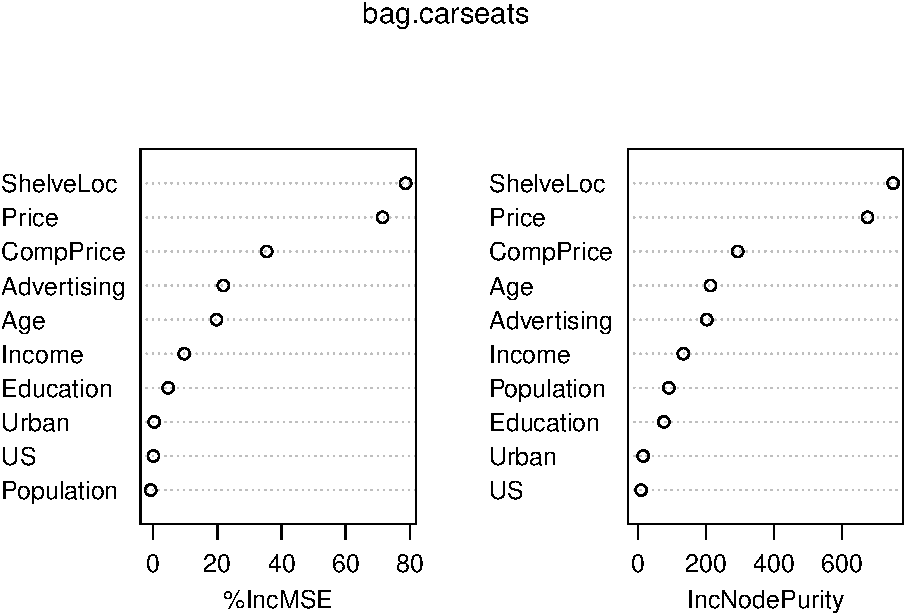
\includegraphics{Disha_Gandhi_Take_Home_Exam_PDF_files/figure-latex/unnamed-chunk-76-1} \end{center}

\begin{itemize}
\item
  As we know, IncMSE and IncNodePurity both should be high for a feature
  to be considered important.
\item
  For our data, \textbf{ShelveLoc, Price, CompPrice, and Age} are all
  important in the respective order as listed. This is also visible from
  the graph where we have plotted these things.
\item
  Also, the MSE on test data is significantly reduced for bagging when
  compared with Regression Trees even after optimization.
\end{itemize}

\hypertarget{part-e-2}{%
\paragraph{\texorpdfstring{{PART E}}{PART E}}\label{part-e-2}}

\begin{verbatim}
## [1] "The  mean square test error in Random Forest is 2.29961839448694"
\end{verbatim}

\begin{verbatim}
##                %IncMSE IncNodePurity
## CompPrice   24.6055514     259.81024
## Income       5.0844785     163.72644
## Advertising 16.6010741     219.46662
## Population   1.9381916     124.67780
## Price       51.5113699     592.37356
## ShelveLoc   58.8389755     686.48012
## Age         16.7074625     245.68816
## Education    1.6325261      92.32343
## Urban       -0.8503112      18.05477
## US           1.9122495      16.14153
\end{verbatim}

\begin{verbatim}
##  [1] 4.844382 3.292354 2.661361 2.404390 2.309417 2.200280 2.199897 2.176413
##  [9] 2.167008 2.231902
\end{verbatim}

\begin{center}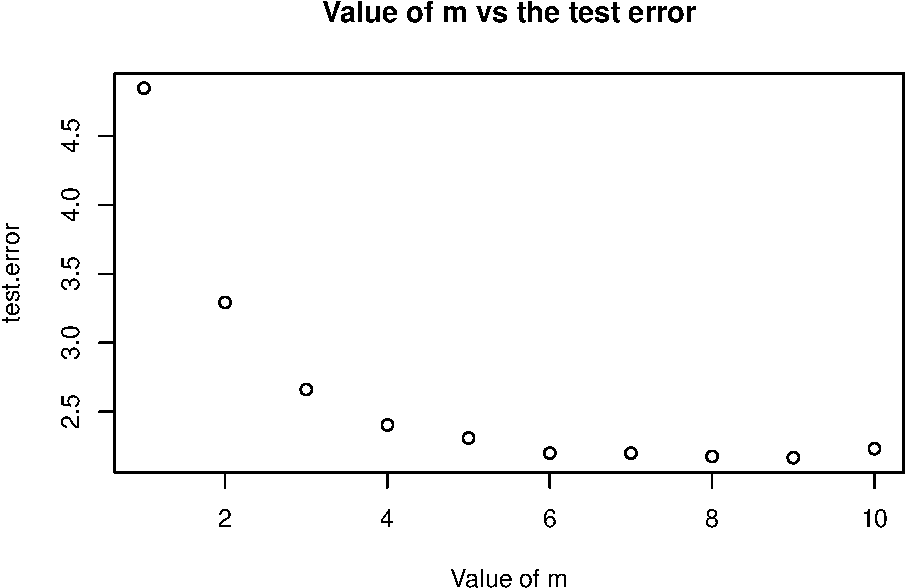
\includegraphics{Disha_Gandhi_Take_Home_Exam_PDF_files/figure-latex/unnamed-chunk-79-1} \end{center}

\begin{itemize}
\item
  Upon looking at the important features in Random Forest we can clearly
  see that the same set of features come at the top that came for other
  regression trees and bagging. Hence we can conclude that all the
  methods give the same set of important features that we listed up.
\item
  I also plotted a graph to show the affect of m on the random forest
  model while evaluating the test error obtained for each iteration. I
  have also listed the test errors for clarity.
\item
  At m=5, the test error is the lowest, and hence I selected that to fit
  my random forest model up.
\item
  But to conclude, we can see that as the value of m increases, the test
  error decreases.
\end{itemize}

\hypertarget{chapter-8-question-11}{%
\subsection{CHAPTER 8 \textasciitilde{} QUESTION
11}\label{chapter-8-question-11}}

\hypertarget{part-a-5}{%
\paragraph{\texorpdfstring{{PART A}}{PART A}}\label{part-a-5}}

\begin{Shaded}
\begin{Highlighting}[]
\FunctionTok{library}\NormalTok{(ISLR)}
\FunctionTok{attach}\NormalTok{(Caravan)}
\NormalTok{train.ind }\OtherTok{=} \DecValTok{1}\SpecialCharTok{:}\DecValTok{1000}
\NormalTok{caravan }\OtherTok{\textless{}{-}}\NormalTok{ Caravan}
\NormalTok{caravan}\SpecialCharTok{$}\NormalTok{Purchase }\OtherTok{=} \FunctionTok{ifelse}\NormalTok{(caravan}\SpecialCharTok{$}\NormalTok{Purchase }\SpecialCharTok{==} \StringTok{"Yes"}\NormalTok{, }\DecValTok{1}\NormalTok{, }\DecValTok{0}\NormalTok{)}
\NormalTok{train }\OtherTok{=}\NormalTok{ caravan[train.ind, ]}
\NormalTok{test }\OtherTok{=}\NormalTok{ caravan[}\SpecialCharTok{{-}}\NormalTok{train.ind, ]}
\end{Highlighting}
\end{Shaded}

\hypertarget{part-b-5}{%
\paragraph{\texorpdfstring{{PART B}}{PART B}}\label{part-b-5}}

\begin{verbatim}
## Warning in gbm.fit(x = x, y = y, offset = offset, distribution = distribution, :
## variable 50: PVRAAUT has no variation.
\end{verbatim}

\begin{verbatim}
## Warning in gbm.fit(x = x, y = y, offset = offset, distribution = distribution, :
## variable 71: AVRAAUT has no variation.
\end{verbatim}

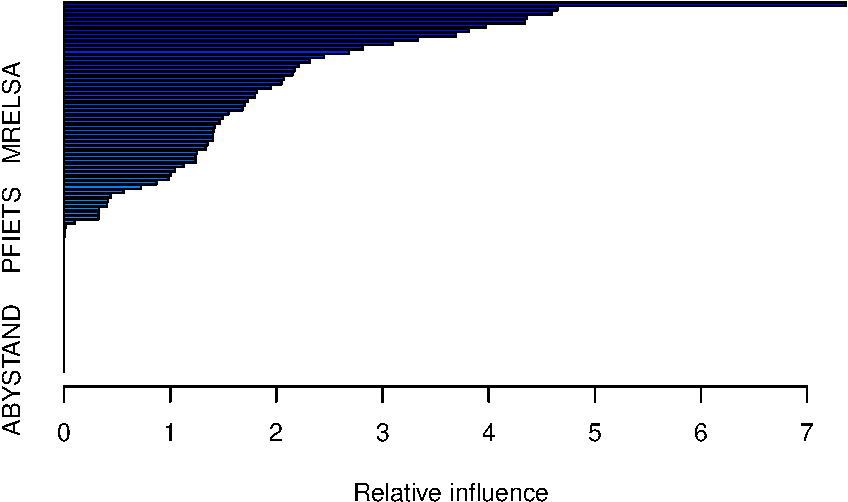
\includegraphics{Disha_Gandhi_Take_Home_Exam_PDF_files/figure-latex/unnamed-chunk-82-1.pdf}

\begin{verbatim}
##               var     rel.inf
## PPERSAUT PPERSAUT 7.360356418
## MKOOPKLA MKOOPKLA 4.647693416
## MGODGE     MGODGE 4.594065009
## MOPLHOOG MOPLHOOG 4.361874298
## MOSTYPE   MOSTYPE 4.342549647
## PBRAND     PBRAND 3.974546766
## MINK3045 MINK3045 3.811079128
## MBERMIDD MBERMIDD 3.690959496
## MGODPR     MGODPR 3.334791636
## MAUT2       MAUT2 3.093196445
## MBERARBG MBERARBG 2.811758220
## MSKC         MSKC 2.683275569
## MFWEKIND MFWEKIND 2.447872903
## PWAPART   PWAPART 2.311346493
## MSKA         MSKA 2.208281221
## MBERHOOG MBERHOOG 2.172366529
## MSKB1       MSKB1 2.148959331
## MINK7512 MINK7512 2.071427618
## MBERARBO MBERARBO 2.048955151
## MINKM30   MINKM30 1.950184599
## MRELOV     MRELOV 1.818306681
## MAUT1       MAUT1 1.798909667
## MRELGE     MRELGE 1.732727293
## MSKB2       MSKB2 1.697615678
## MHHUUR     MHHUUR 1.679969283
## MRELSA     MRELSA 1.546476380
## MOPLMIDD MOPLMIDD 1.492059390
## MFGEKIND MFGEKIND 1.465683906
## MINKGEM   MINKGEM 1.418937155
## MFALLEEN MFALLEEN 1.405908063
## MGEMLEEF MGEMLEEF 1.404465247
## MGODOV     MGODOV 1.400941386
## MZFONDS   MZFONDS 1.348745188
## MAUT0       MAUT0 1.333177135
## ABRAND     ABRAND 1.251191503
## MZPART     MZPART 1.239090497
## MINK4575 MINK4575 1.238084335
## MSKD         MSKD 1.122314443
## MOPLLAAG MOPLLAAG 1.042461254
## MGEMOMV   MGEMOMV 1.001572685
## MGODRK     MGODRK 0.983149208
## MHKOOP     MHKOOP 0.867662192
## APERSAUT APERSAUT 0.725462529
## MOSHOOFD MOSHOOFD 0.557525967
## PMOTSCO   PMOTSCO 0.437553005
## MBERZELF MBERZELF 0.412477909
## PBYSTAND PBYSTAND 0.403310433
## MBERBOER MBERBOER 0.329742638
## PLEVEN     PLEVEN 0.324435477
## MINK123M MINK123M 0.322623169
## MAANTHUI MAANTHUI 0.099896528
## ALEVEN     ALEVEN 0.019411628
## PFIETS     PFIETS 0.006338446
## PWALAND   PWALAND 0.006233808
## PWABEDR   PWABEDR 0.000000000
## PBESAUT   PBESAUT 0.000000000
## PVRAAUT   PVRAAUT 0.000000000
## PAANHANG PAANHANG 0.000000000
## PTRACTOR PTRACTOR 0.000000000
## PWERKT     PWERKT 0.000000000
## PBROM       PBROM 0.000000000
## PPERSONG PPERSONG 0.000000000
## PGEZONG   PGEZONG 0.000000000
## PWAOREG   PWAOREG 0.000000000
## PZEILPL   PZEILPL 0.000000000
## PPLEZIER PPLEZIER 0.000000000
## PINBOED   PINBOED 0.000000000
## AWAPART   AWAPART 0.000000000
## AWABEDR   AWABEDR 0.000000000
## AWALAND   AWALAND 0.000000000
## ABESAUT   ABESAUT 0.000000000
## AMOTSCO   AMOTSCO 0.000000000
## AVRAAUT   AVRAAUT 0.000000000
## AAANHANG AAANHANG 0.000000000
## ATRACTOR ATRACTOR 0.000000000
## AWERKT     AWERKT 0.000000000
## ABROM       ABROM 0.000000000
## APERSONG APERSONG 0.000000000
## AGEZONG   AGEZONG 0.000000000
## AWAOREG   AWAOREG 0.000000000
## AZEILPL   AZEILPL 0.000000000
## APLEZIER APLEZIER 0.000000000
## AFIETS     AFIETS 0.000000000
## AINBOED   AINBOED 0.000000000
## ABYSTAND ABYSTAND 0.000000000
\end{verbatim}

\begin{itemize}
\tightlist
\item
  We can here see the weighted list of features which tell us which
  features are important and which ones are not. Also the features are
  arranged in the decreasing order which will help us in understanding
  their importance.
\item
  The graph is also plotting the same thing. Basically how much does
  each feature influence.
\end{itemize}

\hypertarget{part-c-5}{%
\paragraph{\texorpdfstring{{PART C}}{PART C}}\label{part-c-5}}

After making the predictions, we arrive on the following confusion
matrix for Boosting:

\begin{verbatim}
##    boost.pred
##        0    1
##   0 4355  178
##   1  260   29
\end{verbatim}

\begin{verbatim}
## [1] "The fraction of people predicted to make a purchase and even made one via Boosting is 0.14"
\end{verbatim}

\begin{verbatim}
## Warning: glm.fit: fitted probabilities numerically 0 or 1 occurred
\end{verbatim}

\begin{verbatim}
## Warning in predict.lm(object, newdata, se.fit, scale = 1, type = if (type == :
## prediction from a rank-deficient fit may be misleading
\end{verbatim}

After making the predictions, we arrive on the following confusion
matrix for Logistic Regression:

\begin{verbatim}
##    lm.pred
##        0    1
##   0 4183  350
##   1  231   58
\end{verbatim}

\begin{verbatim}
## [1] "The fraction of people predicted to make a purchase and even made one via Logistic Regression is 0.142"
\end{verbatim}

\begin{itemize}
\tightlist
\item
  We can observe here that the fraction of people predicted to make a
  purchase and even made one is almost similar for both models, Just the
  logistic regression having a 0.2\% greater probability which is
  extremely small. But yes, they're nearly equivalent.
\end{itemize}

\hypertarget{chapter-10-question-7}{%
\subsection{CHAPTER 10 \textasciitilde{} QUESTION
7}\label{chapter-10-question-7}}

We will find both the correlation factor and euclidean distance here for
our dataset and check if the proportionality holds

\begin{verbatim}
##     Min.  1st Qu.   Median     Mean  3rd Qu.     Max. 
## 0.000086 0.069135 0.133943 0.234193 0.262589 4.887686
\end{verbatim}

Upon looking at the summary, we can clearly see here that the
proportionality holds.

\hypertarget{outside-the-textbook-question-1}{%
\subsection{OUTSIDE THE TEXTBOOK \textasciitilde{} QUESTION
1}\label{outside-the-textbook-question-1}}

\hypertarget{part-a-6}{%
\paragraph{\texorpdfstring{{PART A}}{PART A}}\label{part-a-6}}

In order to assess the effect of beauty into course ratings it is
essential for us to first understand the direct relationship between
beauty and course ratings and then evaluate the influence of other
determinants together on the course ratings.

In order to find out the dependency of Course Eval Rating for
instructors we will estimate the effect of BeautyScore by a linear
regression model.

\begin{verbatim}
## 
## Call:
## lm(formula = CourseEvals ~ BeautyScore, data = train)
## 
## Residuals:
##      Min       1Q   Median       3Q      Max 
## -1.59056 -0.32693  0.01846  0.34924  1.23331 
## 
## Coefficients:
##             Estimate Std. Error t value Pr(>|t|)    
## (Intercept)  3.71407    0.02402 154.624   <2e-16 ***
## BeautyScore  0.27721    0.02991   9.267   <2e-16 ***
## ---
## Signif. codes:  0 '***' 0.001 '**' 0.01 '*' 0.05 '.' 0.1 ' ' 1
## 
## Residual standard error: 0.4613 on 368 degrees of freedom
## Multiple R-squared:  0.1892, Adjusted R-squared:  0.187 
## F-statistic: 85.88 on 1 and 368 DF,  p-value: < 2.2e-16
\end{verbatim}

\begin{verbatim}
## [1] "The mean square error of single linear regression model for beauty score is 0.30448986934841"
\end{verbatim}

The p value seems to be less than 0.05 showing statistical significance
and even the SE seems to be on the lower end but the t value is greater
than 2. We will now try multi linear regression model with all the other
features. All the other features seem to be important too and hence to
measure the impact of one while other features are present is also
essential.

\begin{verbatim}
## 
## Call:
## lm(formula = CourseEvals ~ ., data = train)
## 
## Residuals:
##      Min       1Q   Median       3Q      Max 
## -1.30079 -0.30332  0.01142  0.28410  1.03431 
## 
## Coefficients:
##             Estimate Std. Error t value Pr(>|t|)    
## (Intercept)  4.02737    0.05812  69.297  < 2e-16 ***
## BeautyScore  0.30651    0.02723  11.256  < 2e-16 ***
## female      -0.30227    0.04451  -6.791 4.54e-11 ***
## lower       -0.32562    0.04702  -6.926 1.98e-11 ***
## nonenglish  -0.23224    0.09099  -2.552   0.0111 *  
## tenuretrack -0.07577    0.05469  -1.386   0.1667    
## ---
## Signif. codes:  0 '***' 0.001 '**' 0.01 '*' 0.05 '.' 0.1 ' ' 1
## 
## Residual standard error: 0.416 on 364 degrees of freedom
## Multiple R-squared:  0.3477, Adjusted R-squared:  0.3387 
## F-statistic:  38.8 on 5 and 364 DF,  p-value: < 2.2e-16
\end{verbatim}

\begin{verbatim}
## [1] "The mean square error of multi linear regression model for all features is 0.221653402571502"
\end{verbatim}

We can clearly see here that the coefficients are both negative and
positive which is obvious as as if a professor is not a native English
speaker, he/she will have problems communicating to the class about the
course leading to less productivity. Whereas a negative coefficient in
female feature should not be there. This hints us that there might be a
bias to rate female instructors less which might be just a bias or there
might be genuine issues in understanding those courses. We can only
speculate here. But this data does tell us that beauty has a positive
coefficient for course ratings which means that it influences
productivity to an extent but the coefficient is similar in weightage to
other features and so it is not one of the dominating features. The p
value here too seems to be less than 0.05 showing statistical
significance and the accuracy has just improved while the mean square
error dropping significantly. This shows us that Multi linear regression
model is a better fit compared to single.

For further insights, I have also tried to fit partial least squares:

\begin{center}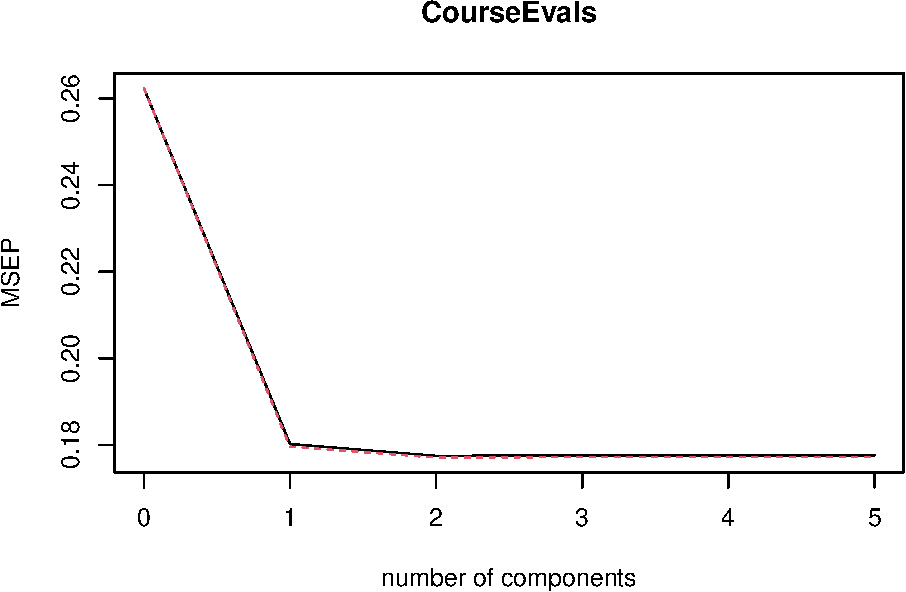
\includegraphics{Disha_Gandhi_Take_Home_Exam_PDF_files/figure-latex/unnamed-chunk-96-1} \end{center}

\begin{verbatim}
## [1] "The mean square error of partial least squares regression model for all features is 0.221828055974601"
\end{verbatim}

The mean square error in this case is very similar to the error obtained
in multi linear regression model. Hence both seem to fit very well and
give us a relation between course evals and other determinants.

\hypertarget{part-b-6}{%
\paragraph{\texorpdfstring{{PART B}}{PART B}}\label{part-b-6}}

\begin{verbatim}
## [1] "The correlation between beauty score and course ratings is 0.43"
\end{verbatim}

\begin{itemize}
\item
  The question being asked in this paper is whether the Beauty quotient
  of an instructor genuinely increases the productivity of students in
  their courses or it is just a bias in the mind of students that causes
  a cloud of judgement and makes them give ratings without any logical
  conclusion.
\item
  When we ran our regression model we saw that beauty has a positive
  impact but it is not that significant to declare that it alone is an
  influence in the increase in ratings for an instructor. The
  correlation above between beauty and ratings feature show a slight
  positive correlation which might cause a small collinearity between
  them thus influencing the regression fit.
\item
  Now even if beauty is influencing, it might be that beauty increases a
  person's self confidence and hence causes them to communicate better
  and effectively. Or it can also be true that the natural human bias
  forces a person to discriminate and give better ratings to good
  looking professors. We can only conclude on this if we are 100\% sure
  that our audience is unbiased and hence the direct proportionality of
  beauty score is purely related to increase in productivity. And for
  this we need to generate the target data set differently in different
  conditions.
\item
  Beauty should ideally not be an important factor in determining the
  ability of a professor to teach well. But as our results show that it
  is an important feature then these ratings should not be the grounds
  for an economic decision.
\end{itemize}

\hypertarget{outside-the-textbook-question-2}{%
\subsection{OUTSIDE THE TEXTBOOK \textasciitilde{} QUESTION
2}\label{outside-the-textbook-question-2}}

To answer part A and B we need to encode brick column and also generate
two new columns N2 and N3 so that we fit them and generate analysis.

After generating the required columns, we fit a multi linear regression
model and check the coefficients for the required features to check for
null hypothesis.

\begin{verbatim}
## 
## Call:
## lm(formula = Price ~ Offers + SqFt + Brick + Bedrooms + Bathrooms + 
##     N2 + N3, data = midcity.df)
## 
## Residuals:
##      Min       1Q   Median       3Q      Max 
## -27337.3  -6549.5    -41.7   5803.4  27359.3 
## 
## Coefficients:
##              Estimate Std. Error t value Pr(>|t|)    
## (Intercept)  2159.498   8877.810   0.243  0.80823    
## Offers      -8267.488   1084.777  -7.621 6.47e-12 ***
## SqFt           52.994      5.734   9.242 1.10e-15 ***
## Brick       17297.350   1981.616   8.729 1.78e-14 ***
## Bedrooms     4246.794   1597.911   2.658  0.00894 ** 
## Bathrooms    7883.278   2117.035   3.724  0.00030 ***
## N2          -1560.579   2396.765  -0.651  0.51621    
## N3          20681.037   3148.954   6.568 1.38e-09 ***
## ---
## Signif. codes:  0 '***' 0.001 '**' 0.01 '*' 0.05 '.' 0.1 ' ' 1
## 
## Residual standard error: 10020 on 120 degrees of freedom
## Multiple R-squared:  0.8686, Adjusted R-squared:  0.861 
## F-statistic: 113.3 on 7 and 120 DF,  p-value: < 2.2e-16
\end{verbatim}

\hypertarget{part-a-7}{%
\paragraph{\texorpdfstring{{PART A}}{PART A}}\label{part-a-7}}

This part requires us to evaluate if brick houses cause a premium and so
we will have to isolate the coefficient for brick houses and get the
confidence interval using the above model fit.

\begin{verbatim}
##          2.5 %   97.5 %
## Brick 13373.89 21220.81
\end{verbatim}

We can see here that 95\% confidence interval for coefficient of Brick
houses is {[}13373.89, 21220.81{]}. Now since 0 is not present in this
confidence interval, we can reject the null hypothesis that coefficient
of Brick houses will be zero anytime and so brick house is an important
feature with statistical significance that generates a premium. It's
value will never be negative and hence there will always be a premium.

\hypertarget{part-b-7}{%
\paragraph{\texorpdfstring{{PART B}}{PART B}}\label{part-b-7}}

This part requires us to evaluate if Neighborhood 3 cause a premium and
so we will have to isolate the coefficient for Neighborhood 3 and get
the confidence interval using the above model fit.

\begin{verbatim}
##       2.5 %   97.5 %
## N3 14446.33 26915.75
\end{verbatim}

We can see here that 95\% confidence interval for coefficient of
Neighborhood 3 is {[}14446.33, 26915.75{]}. Now since 0 is not present
in this confidence interval, we can reject the null hypothesis that
coefficient of Neighborhood 3 will be zero anytime and so living in
Neighborhood 3 is an important feature with statistical significance
that generates a premium. People living in Neighborhood 3 will always
pay extra since the premium is positive.

\hypertarget{part-c-6}{%
\paragraph{\texorpdfstring{{PART C}}{PART C}}\label{part-c-6}}

This part requires us to evaluate if Neighborhood 2 and Neighborhood 1
can be merged into older neighborhood. If N2 is not statistically
significant then we can declare it as not important. Hence we will check
the null hypothesis for N2 by looking at it's confidence interval.

\begin{verbatim}
##        2.5 %  97.5 %
## N2 -6306.008 3184.85
\end{verbatim}

After looking at the confidence interval for N2 {[}???6306, 3184{]}, we
can clearly see that 0 lies in this range and hence we cannot reject the
null hypothesis. Therefore Neighborhood 2 can be merged with
Neighborhood 1 because in certain cases it might not be significant and
in those cases Neighborhood 1 can play it's role.

\hypertarget{part-c-7}{%
\paragraph{\texorpdfstring{{PART C}}{PART C}}\label{part-c-7}}

To evaluate the premium generated by brick houses in neighborhood 3, we
will have to write a new feature formed by an and operation on brick and
neighborhood 3. After generating this feature we will again fit a multi
linear regression model with all of the previously selected features
plus this one and then again look at the confidence interval for this
feature on the fitted model.

\begin{verbatim}
## 
## Call:
## lm(formula = Price ~ Offers + SqFt + Brick + Bedrooms + Bathrooms + 
##     N2 + N3 + BrickN3, data = midcity.df)
## 
## Residuals:
##      Min       1Q   Median       3Q      Max 
## -26939.1  -5428.7   -213.9   4519.3  26211.4 
## 
## Coefficients:
##              Estimate Std. Error t value Pr(>|t|)    
## (Intercept)  3009.993   8706.264   0.346  0.73016    
## Offers      -8401.088   1064.370  -7.893 1.62e-12 ***
## SqFt           54.065      5.636   9.593  < 2e-16 ***
## Brick       13826.465   2405.556   5.748 7.11e-08 ***
## Bedrooms     4718.163   1577.613   2.991  0.00338 ** 
## Bathrooms    6463.365   2154.264   3.000  0.00329 ** 
## N2           -673.028   2376.477  -0.283  0.77751    
## N3          17241.413   3391.347   5.084 1.39e-06 ***
## BrickN3     10181.577   4165.274   2.444  0.01598 *  
## ---
## Signif. codes:  0 '***' 0.001 '**' 0.01 '*' 0.05 '.' 0.1 ' ' 1
## 
## Residual standard error: 9817 on 119 degrees of freedom
## Multiple R-squared:  0.8749, Adjusted R-squared:  0.8665 
## F-statistic:   104 on 8 and 119 DF,  p-value: < 2.2e-16
\end{verbatim}

\begin{verbatim}
##            2.5 %   97.5 %
## BrickN3 1933.918 18429.24
\end{verbatim}

As we can see that the confidence interval for Brick houses in
Neighborhood 3 is {[}1933.91, 18429.24{]}. There is no 0 in the range
and so we can reject the null hypothesis. That implies that people are
ready to pay extra premium/price for a brick house in neighborhood 3.

\hypertarget{outside-the-textbook-question-3}{%
\subsection{OUTSIDE THE TEXTBOOK \textasciitilde{} QUESTION
3}\label{outside-the-textbook-question-3}}

\hypertarget{part-a-8}{%
\paragraph{PART A}\label{part-a-8}}

Even if we get the data from different cities on the crime rate and the
police deployed on the streets, \textbf{we never will be able to
identify the causal relationship between them. i.e what caused what.} It
is possible that more crime led to more police being deployed or more
police is leading to increased crime. In order to actually find the
dependency between them, hypothetical scenarios will have to be created
where in we can evaluate that keeping other determinants/features
constant who influences who. Obviously creating such scenarios is
practically not possible. Hence simply running the regression on these
both won't give any significant results \textbf{until we can simulate
favorable situations} to generate data that answers the above question
first.

\hypertarget{part-b-8}{%
\paragraph{\texorpdfstring{{PART B}}{PART B}}\label{part-b-8}}

The researchers at UPENN helped us by \textbf{creating a simulated
natural environment} for which if we collect data we can actually
\textbf{answer the relationship between crime and police.} On one of the
potential high alert days due to terror threats, the mayor deployed more
police. So technically more police was deployed and we could now assess
it's impact on crime rate. \textbf{Their approach:} They controlled two
features, ridership in metro, and the number of police. They both have a
negative relationship with the crime rate as visible in Table 2
\textbf{(negative coefficient).} So you never know if the crime is
reduced that is because of less people in the metros(more control on
ridership) or more number of police deployed on the streets.

\hypertarget{part-c-8}{%
\paragraph{\texorpdfstring{{PART C}}{PART C}}\label{part-c-8}}

In order to find out the effect of number of police, it is essential to
consider other possible features too on crime rate. Because if we have
to isolate the police strength we have to determine the coefficient of
other possible determinants. One of them is less number of people which
happens on high alert days and controlling ridership can simulate that.
Now on high alert days police strength increases and crime reduces but
along with that number of people on street is also reducing.

Because of the reduce in the number of people on the street, it is also
possible that even the criminals won't choose to step out thus reducing
the crime rate. So even in this simulated situation more number of
people might not be the cause for reduced crime rate even though they
share a negative association. Hence it was essential for them to control
metro ridership to account for this factor.

\hypertarget{part-d-4}{%
\paragraph{\texorpdfstring{{PART D}}{PART D}}\label{part-d-4}}

Table 4 is measuring the \textbf{effect of high alert days and the above
analysis in different regions of Washington DC}. The coefficient for
district 1 is higher than other districts maybe because district 1 has a
higher threat causing the mayor to deploy more police over there or
maybe some other reason causing the crime rate to reduce much more. None
the less \textbf{both have a negative coefficient} implying an overall
reduction in the crime rate.

\hypertarget{outside-the-textbook-question-4}{%
\subsection{OUTSIDE THE TEXTBOOK \textasciitilde{} QUESTION
4}\label{outside-the-textbook-question-4}}

\hypertarget{my-contribution-in-the-final-group-project}{%
\subparagraph{\texorpdfstring{\textbf{My Contribution in the Final Group
Project}}{My Contribution in the Final Group Project}}\label{my-contribution-in-the-final-group-project}}

\begin{itemize}
\item
  With a very interesting dataset on regression problem we started our
  brainstorming session on how to approach the problem. But upon looking
  at it closely we found out that it is not competitive enough and so we
  again searched a dataset from the available options, 2 options
  provided by each member including me. We finalized on the credit
  history tracking and credit approval classification problem.
\item
  The challenge was to use a logic to convert the credit history to
  ideal buckets for classification. Over here my suggestion was to
  consider 3 buckets, 0(good guys), 1(defaulting guys but paying it in a
  while), and 2(bad guys not paying). But for the sake of simplicity we
  went ahead with only 2 buckets, 0(good guys) and 1(bad guys).
\item
  Next task was to study the data and perform EDA so that we can fit the
  right model. I did the missing value analysis and all the required
  encoding. We used get\_dummies function from python for encoding the
  categorical data as it uses n-1 bits over one hot encoding.
\item
  We all took multiple iterations to understand and perform uni-variate
  and bivariate analysis till we could come together on the right set of
  features which were correlated to the credit approval feature.
\item
  After splitting the train and test data along with a validation set
  into 80:20, I moved to implementing Random Forest Algorithm to
  classify the credit history feature. Others similarly took one model
  each for implementation.
\item
  At first I implemented plain vanilla Random Forest Algorithm and
  checked the confusion matrix and recall score. We had decided to focus
  on recall score because according to our use case solving the Type 1
  error was our priority. The bank may miss out good potential customers
  and the corresponding revenue from them but it should not lend the
  money to wrong customers. Hence our target was to optimize recall
  obtained here. In this approach we received a recall of 0.04 which was
  very bad.
\item
  I then performed Random grid search CV to do hyper parameter tuning
  for my model and observed a very small increase in the recall score
  which was not a big motivation. Here I learnt about various parameters
  present in Random Forest Algorithm and how to ideally fit them into
  the model.
\item
  I further also plotted feature importance and probability distribution
  function(PDF). In the feature importance graph, I could see a stark
  similarity in the top features here and what we observed in bivariate
  analysis. That's when we knew we are on the right line. Our PDF showed
  us the overlapping of both buckets and that we will have to reduce our
  threshold to as low as 0.13 if we want significant classification.
\item
  Once everyone was done with their implementation, we concluded a final
  model and converted our jupyter cells into slides for presentation and
  prepared for our respective parts.
\item
  Some of the essential lessons I learnt were, trees and their
  optimization, random grid search, importance of cross validation,
  bivariate analysis. And some obvious lessons like team work,
  segregation of duties, collaboration on presentations, even virtually
  for that case.
\end{itemize}

\end{document}
